%\texorpdfstring{}
\documentclass[review]{elsarticle}
\usepackage{lineno}
\usepackage{amssymb}
\usepackage{amsmath}
\usepackage{booktabs}
\usepackage{siunitx}
\usepackage{enumitem}
\usepackage{graphicx}
\usepackage{float}
\usepackage{placeins}
\usepackage{dblfloatfix}
\usepackage{xcolor}
\definecolor{mgGreen}{HTML}{2CA02C} % matches SOC/SOH "Base" colour in plots
\definecolor{mgRed}{HTML}{D62728}   % matches "Pruned" / red tone in plots
\usepackage{hyperref}
\journal{Engineering Applications of Artificial Intelligence}
\date{}
\newcommand{\code}[1]{\path{#1}}
\newcommand{\benchfig}[2]{%
\IfFileExists{#1}{\includegraphics[width=\columnwidth]{#1}}{\fbox{\parbox{0.9\columnwidth}{#2\\\path{#1}}}}%
}
\newcommand{\aitodo}[1]{\textcolor{red}{[TODO: #1]}}     % assistant-facing notes (visible)
\makeatletter
% Float tuning: reduce figure-only pages and allow more organic text/figure interleaving.
\renewcommand{\topfraction}{0.85}
\renewcommand{\bottomfraction}{0.85}
\renewcommand{\textfraction}{0.15}
\renewcommand{\floatpagefraction}{0.90}
\renewcommand{\dbltopfraction}{0.85}
\renewcommand{\dblfloatpagefraction}{0.90}
\setcounter{topnumber}{2}
\setcounter{bottomnumber}{2}
\setcounter{totalnumber}{4}
\setcounter{dbltopnumber}{2}
\makeatother

% Reduce vertical white-space stretching on pages with large floats.
\raggedbottom

% The paper does not use List of Figures/Tables. Disabling writes to `lof/lot`
% keeps auxiliary files small and avoids sporadic NUL-byte corruption on
% synced/networked folders during repeated LaTeX runs.
\makeatletter
\let\orig@addcontentsline\addcontentsline
\def\addcontentsline#1#2#3{%
  \def\@tempa{#1}%
  \def\@tempb{lof}%
  \def\@tempc{lot}%
  \ifx\@tempa\@tempb\else
    \ifx\@tempa\@tempc\else
      \orig@addcontentsline{#1}{#2}{#3}%
    \fi
  \fi
}

% Avoid writing long caption strings into `soc_outline.aux` (not needed; the
% paper does not use `\nameref`). This significantly reduces aux file size.
\let\orig@caption\@caption
\long\def\@caption#1[#2]#3{%
  \orig@caption#1[#2]{#3}%
  \gdef\@currentlabelname{}%
}
\makeatother
\begin{document}
\linenumbers
\begin{frontmatter}
\title{Embedded Artificial Intelligence in Battery Management Systems: Pruning and Quantization for Efficient State-of-Charge and State-of-Health Estimation}
\author{Anonymous}
\affiliation{organization={Anonymous}}
\begin{abstract}
State-of-charge (SOC) and state-of-health (SOH) estimators based on recurrent neural networks can achieve high accuracy, but their computational and memory cost on embedded hardware is often insufficiently characterised. This work quantifies the accuracy, timing, and resource trade-offs of Long Short-Term Memory (LSTM) and Multi-Layer Perceptron (MLP) based SOC/SOH estimators deployed on an STM32H753ZI microcontroller. Using the open \emph{Lithium Iron Phosphate (LFP) Cycle Ageing Dataset}, we train full-precision baseline models and obtain compressed variants via pruning and weight quantization. In long-horizon streaming replay on the test set the SOC estimators attain mean-absolute errors (MAE) between $2.3$~\% and $2.8$~\% of full scale, while the SOH estimators reach MAE values between $0.9$~\% and $1.5$~\%. Hardware-in-the-loop benchmarks on the STM32 show that pruning reduces both the flash footprint and the energy per inference by roughly $40$~\% for SOC and about $45$~\% for SOH, while slightly improving SOC MAE and keeping SOH MAE within a few tenths of a percent of the dense baseline. Quantization further shrinks the flash footprint to around half of the baseline size for both tasks and keeps the MAE within a few tenths of a percent of the corresponding full-precision models, at the expense of increased inference energy, especially for SOC. The presented methodology and measurements provide a reproducible reference for implementing and comparing data-driven battery state estimators on resource-constrained Battery Management System (BMS) hardware.
\end{abstract}
\begin{keyword}
State of charge \sep State of health \sep Long short-term memory \sep Pruning \sep Quantization \sep Microcontroller \sep Battery diagnostics \sep Embedded artificial intelligence
\end{keyword}
\end{frontmatter}
\section*{Nomenclature}
\small
\subsection*{Acronyms}
\begin{description}[style=multiline,leftmargin=1.5cm,font=\bfseries]
\item[BMS] Battery management system
\item[SOC] State of charge
\item[SOH] State of health
\item[DoE] Design of Experiments
\item[LFP] Lithium iron phosphate
\item[LSTM] Long short-term memory network
\item[MLP] Multi-layer perceptron
\item[STM32] 32-bit ARM Cortex-M microcontroller family
\item[MAE] Mean absolute error
\item[RMSE] Root-mean-square error
\item[INT8] Signed 8-bit integer representation (quantized weights)
\item[FP32] 32-bit floating-point representation
\end{description}
\medskip
\subsection*{Symbols}
\begin{description}[style=multiline,leftmargin=1.5cm,font=\bfseries]
\item[$t$] Time
\item[$U(t)$] Terminal voltage at time $t$
\item[$I(t)$] Current at time $t$ (positive for discharge)
\item[$T(t)$] Cell temperature at time $t$
\item[$\mathrm{EFC}(t)$] Equivalent full cycles accumulated up to $t$
\item[$Q_c(t)$] Cumulative charge throughput up to $t$
\item[$C_{\mathrm{nom}}$] Nominal discharge capacity of the cell
\item[$C_{\mathrm{app}}$] Apparent capacity inferred from the latest check-up
\item[$\mathrm{DoD}$] Depth of discharge
\item[$\mathrm{SOC}(t)$] State of charge at time $t$
\item[$\mathrm{SOH}_k$] State of health at reference cycle $k$
\item[$\mathbf{x}_t$] Input feature vector at time $t$
\item[$\mathbf{h}_t$] LSTM hidden state at time $t$
\item[$\mathbf{c}_t$] LSTM cell state at time $t$
\item[$\mathbf{z}_t$] Concatenation of input and previous hidden state at time $t$
\item[$\mathbf{i}_t,\mathbf{f}_t,\mathbf{o}_t,\mathbf{g}_t$] Input, forget, output, and candidate gates at time $t$
\item[$\sigma(\cdot)$] Logistic sigmoid activation function
\item[$\tanh(\cdot)$] Hyperbolic tangent activation function
\item[$\odot$] Element-wise (Hadamard) product
\item[$W$] Weight matrix (LSTM or MLP)
\item[$b$] Bias vector
\item[$q$] Quantized weight (INT8 code)
\item[$s$] Per-row quantization scale (FP32)
\item[$\hat{w}$] Reconstructed floating-point weight after dequantization
\item[$\mathcal{Q}_s(\cdot)$] Uniform mid-tread quantizer with scale $s$
\item[$W_{\mathrm{ih}}^{\mathrm{int8}}$] Quantized input-to-gate weight matrix
\item[$W_{\mathrm{hh}}^{\mathrm{int8}}$] Quantized hidden-to-gate weight matrix
\item[$s_{\mathrm{ih}}, s_{\mathrm{hh}}$] Per-row quantization scale vectors for $W_{\mathrm{ih}}^{\mathrm{int8}}$ and $W_{\mathrm{hh}}^{\mathrm{int8}}$
\item[$b_{\mathrm{fp32}}$] Floating-point bias of a given gate
\item[$g$] Gate pre-activation used in the quantized LSTM kernel
\end{description}
\normalsize
\section{Introduction}
Accurate online estimation of the state of charge (SOC) and the state of health (SOH) remains a central challenge for battery powered systems~\cite{yaoSmarterBatteryManagement2025a,a.m.s.m.h.s.attanayakaEstimationStateCharge2019,berecibarCriticalReviewState2016,shrivastavaReviewTechnologicalAdvancement2023}. Classical model-based estimation schemes often struggle to track long-term degradation under highly dynamic current and temperature conditions. Neural networks can capture such effects and have recently been surveyed comprehensively for SOC estimation in~\cite{yaoSmarterBatteryManagement2025a}, yet the majority of published solutions remain purely theoretical: they report accuracy on offline datasets but rarely demonstrate how the models behave once deployed on embedded targets with tight memory and energy budgets. This work closes this gap by optimising SOC and SOH Long Short-Term Memory (LSTM) models for microcontroller deployment using pruning and quantization.
The methodology is motivated by modular stationary storage systems in remote microgrids, where battery storage modules must operate autonomously without reliable infrastructure. In such settings, the battery management system must compute SOC and SOH within the flash, RAM, and energy limits of an STM32H753ZI-class microcontroller. Similar demands arise in mobile applications where devices must run for long periods without cloud support. Translating high-fidelity neural estimators into this environment is therefore an enabling step for future resource-aware Battery Management System (BMS) platforms.
While many machine-learning models for state estimation have been proposed~\cite{yaoSmarterBatteryManagement2025a}, accompanying artefacts such as scaling statistics, hidden-state handling, and quantization parameters are rarely documented in sufficient detail to enable faithful reproduction on microcontrollers. Even fewer works report resource usage, energy consumption, or long-horizon streaming behaviour of the deployed models, with only a handful of studies analysing Tiny Machine Learning (TinyML)-style SOC or SOH estimators on microcontrollers~\cite{crocioniLiIonBatteriesParameter2020,Embedded_AI_only_SOC_mobile,Embedded_AI_SOH_badData}. Against this backdrop, we focus on closing the gap between theoretical validation and embedded deployment, with a particular emphasis on optimisation for memory, runtime, and energy.
In the remainder of this work we rely on the resulting Lithium Iron Phosphate (LFP) DoE Cycle Ageing Dataset~\cite{LFP_DoE_Cycle_Aging_Dataset}. The data capture long-term cyclic ageing of numerous LFP cells under full and fractional factorial conditions with controlled temperature, charge and discharge rates, depth-of-discharge variations, and interleaved check-ups containing capacity tests, OCV sweeps, and hybrid pulse-power characterisation. This breadth provides a realistic basis for training and evaluating SOC and SOH estimators across a wide range of ageing patterns.
\section{Related Work and Motivation}
\subsection{SOC/SOH Estimation}
Existing SOC/SOH estimation methods can be grouped into three families~\cite{a.m.s.m.h.s.attanayakaEstimationStateCharge2019,berecibarCriticalReviewState2016,shrivastavaReviewTechnologicalAdvancement2023,guoSystematicReviewElectrochemical2024}. First, \emph{measurement-derived} techniques use Coulomb counting and open-circuit-voltage (OCV) look-up tables during rest periods. They provide inexpensive proxies but suffer from drift, offset accumulation, and a strong dependence on initialisation and periodic recalibration. Second, \emph{model-based} observers combine equivalent-circuit or electrochemical models with Kalman filtering and its variants. These approaches can offer physical interpretability but require careful parameter identification and are sensitive to model mismatch and ageing-induced parameter drift. Third, \emph{data-driven} methods employ machine-learning regressors, including LSTM networks, Transformers, and hybrid structures, to map sequences of current, voltage, and temperature to SOC and SOH estimates. Key challenges for such models are robustness when operated under conditions that differ from the training data and the careful treatment of normalisation and state handling on embedded targets.
Across these families the reported accuracy spans a wide range. Electrochemical or Equivalent Circuit Model (ECM)-based observers with carefully tuned filters often achieve SOC root-mean-square errors (RMSE) well below $1\,\%$ of full scale and sub-percent SOH capacity errors on laboratory test cycles~\cite{gaoCoEstimationStateofChargeStateof2022,gaoEnhancedStateofchargeEstimation2022,shenAlternativeCombinedCoestimation2022,wangFusionEstimationLithiumion2022}. Recent sequence-model approaches based on N-BEATS and Bidirectional LSTMs (BiLSTMs) for sodium-ion cells report SOC Mean Absolute Error (MAE) between roughly $0.1$ and $0.4\,\%$~\cite{sunStateChargeEstimation2023,sunStateofchargeEstimationSodiumion2024}, whereas TinyML-style SOC estimators deployed on microcontrollers typically operate in the 1--3~\% error regime~\cite{crocioniLiIonBatteriesParameter2020,giazitzisCaseStudyTiny2024,Embedded_AI_only_SOC_mobile}. These results provide a useful reference band for the SOC/SOH errors obtained in this work.
Kalman filters, particle filters, and equivalent-circuit-model observers therefore dominate the classical literature, yet their accuracy can degrade over long operating periods with pronounced current and temperature gradients~\cite{gaoEnhancedStateofchargeEstimation2022,wangFusionEstimationLithiumion2022}. Recurrent neural networks, and in particular LSTM-based regressors, address these limitations by integrating long temporal context and absorbing residual modelling errors~\cite{liOnlineCapacityEstimation2021,wangFusionEstimationLithiumion2022}. In this work we deliberately restrict the architecture search to a single-layer LSTM with a fully connected Multi-Layer Perceptron (MLP) output layer. LSTMs retain explicit cell states with separate input, forget, and output gates, which made it straightforward to hand-code a numerically stable, stateful kernel in C and to reuse the same backbone for both SOC and SOH. Gated recurrent units (GRUs) or Transformer variants could offer alternative trade-offs between accuracy and cost, but exploring multiple architectures would dilute the focus on the embedded tool flow and is left as future work.
Most publications on LSTM-based estimators maximise accuracy with complex architectures and rarely examine how the resulting models behave once deployed on constrained controllers. Even within the LSTM family, sliding-window inference is commonly employed because it delivers high accuracy, but it also requires substantial RAM to buffer multiple past samples. A stateful LSTM that hands over its hidden and cell vectors step by step retains the temporal information without maintaining large windows and therefore forms the first optimisation step in our architecture. The associated handling of hidden states, feature scaling, and numerical stability is rarely described in the literature, which is why this work explicitly targets embedded SOC/SOH deployment.
\begin{figure*}[t!]
    \centering
    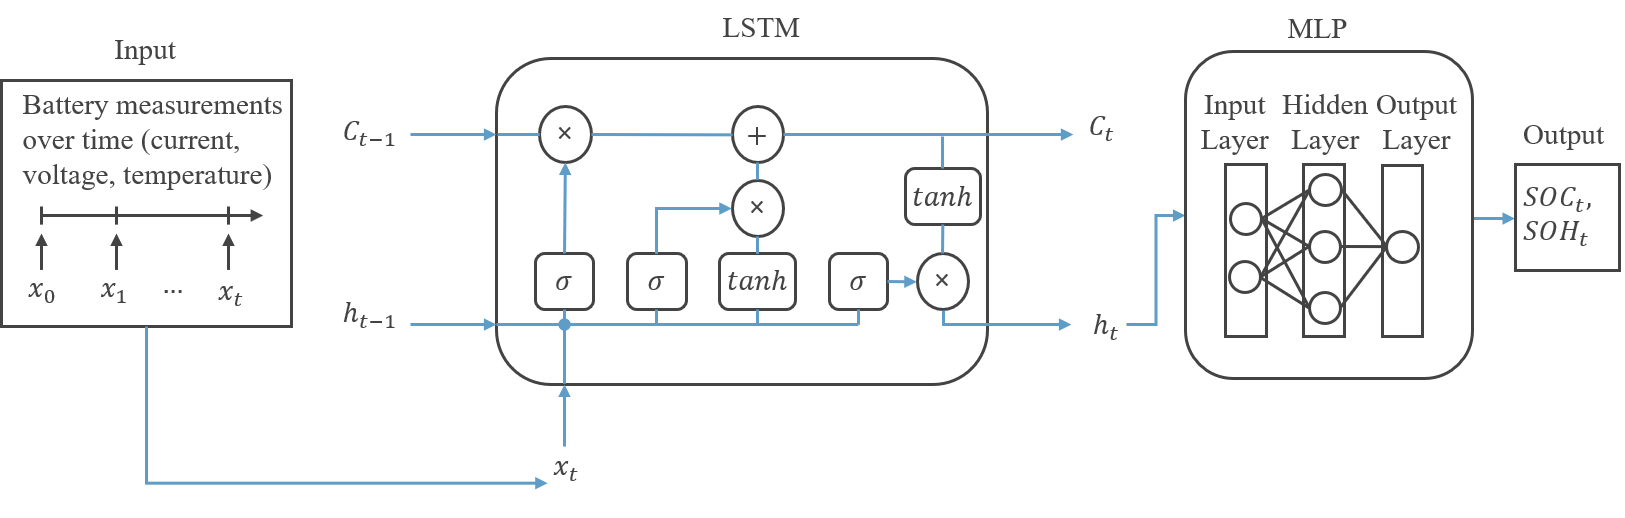
\includegraphics[width=\textwidth]{figures/Schematics/Figure_1_LSTM_MLP_Schematic.png}
    \caption[Stateful LSTM+MLP estimator]{Schematic of the deployed SOC/SOH estimator. Preprocessed feature streams are fed into a single-layer LSTM whose hidden state is propagated across time; at each step a lightweight MLP head maps the hidden representation either to SOC or SOH, enabling stateful streaming inference on the STM32.}
    \label{fig:lstm_mlp_schematic}
\end{figure*}
\subsection{Embedded Deployment Strategies}
Commercial toolchains such as ONNX Runtime, TensorRT, and STM32Cube.AI can export many feed-forward networks~\cite{ONNXRuntimeHighperformance,NVIDIATensorRTHighPerformance,XCUBEAISTM32CubeExpansion}, but they fall short for stateful SOC/SOH estimators that must maintain continuous internal states between time steps. In addition, safety-critical deployments require predictable behaviour and source code that can be audited, which is difficult when quantization and optimisation are hidden inside proprietary binaries. Besides the stateful execution, embedded operation also demands explicit control over footprint, hence pruning and quantization must be applied in a transparent way rather than via opaque compiler passes. Complementary work such as~\cite{naguibMicroprocessorExecutionTime2022} quantifies execution time and memory for a variety of SOC algorithms on microcontrollers, while PQ Bench~\cite{schulzePQBenchBenchmarking2025} provides a systematic benchmark of modern pruning and quantization techniques and demonstrates that they can deliver strong compression--accuracy trade-offs across diverse deep-learning workloads. Our study builds on these insights by applying pruning and quantization to stateful LSTM\,+\,MLP SOC/SOH estimators and by extending the analysis to a full STM32 firmware implementation with detailed measurements of flash, RAM, latency, and energy in a realistic BMS setting. We therefore opted for a manual path: extracting PyTorch tensors, pruning rows and columns according to saliency, applying per-row symmetric quantization for the LSTM weights, and re-implementing the gates and activations in plain C. This guarantees that every multiplication, scaling, and bias term seen on the STM32 matches the reference simulation while keeping the model within the available RAM and flash budgets.
\section{Dataset and Preprocessing}
\subsection{Ageing Experiments and Load Profiles}
All experiments rely on the high-resolution LFP DoE Cycle Ageing Dataset~\cite{LFP_DoE_Cycle_Aging_Dataset}. The measurements originate from a design-of-experiments study on commercially available JGCFR18650-1800mAh-3.2V LFP cells~\cite{jgneJGCFR186501800mAh32VProductSpecification} conducted in a university laboratory. Cells were cycled inside a climatic chamber at $25^\circ\mathrm{C}$ while the following factors were systematically varied:
\begin{align}
    C_{\mathrm{chg}} &\in [0.5\,\mathrm{C},\,0.9\,\mathrm{C}],\\
    C_{\mathrm{dis}} &\in [1.0\,\mathrm{C},\,2.5\,\mathrm{C}],\\
    \mathrm{DoD} &\in [45\%,\,65\%].
\end{align}
A mixed full/fractional factorial plan assigned fifteen test cells to eight operating points, each condition being executed in duplicate to ensure reproducibility. Between ageing loops, dedicated check-ups consisting of capacity tests, open-circuit-voltage sweeps, and hybrid pulse power characterisation were inserted to parameterise the cells. In addition to the strictly controlled cycling sequences, stationary-storage profiles were injected to emulate realistic power flows~\cite{kucevicStandardBatteryEnergy2020a}. These profiles are derived from residential photovoltaic (PV) home storage applications, which are characterised by stochastic load and generation patterns that stress the cell dynamics differently than constant-current cycling. The raw data contain uniformly sampled (1~Hz) measurements of voltage, current, terminal temperature, and auxiliary channels and are stored as partitioned Parquet tables for efficient retrieval.
\begin{figure}[htbp]
    \centering
    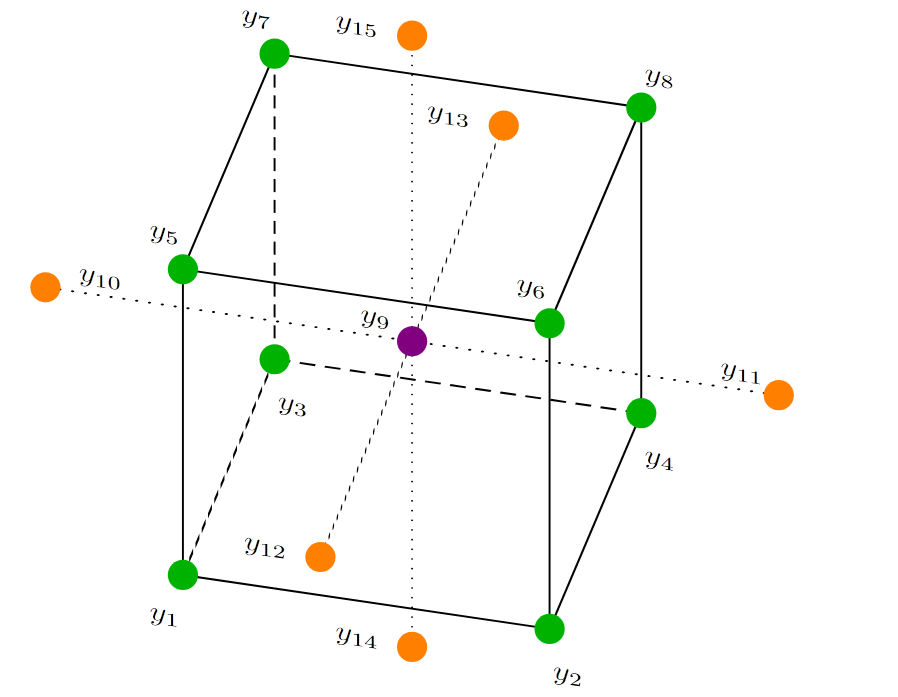
\includegraphics[width=\columnwidth]{figures/Schematics/Figure_2_DoE_Cube.png}
    \caption[Design-of-experiments cube]{Design-of-experiments cube for the LFP DoE Cycle Ageing Dataset. The three axes correspond to charge C-rate, discharge C-rate, and depth of discharge (DoD); the highlighted vertices indicate the eight factorial operating points assigned to the test cells.}
    \label{fig:doe_cube}
\end{figure}
\noindent The dataset is published in~\cite{LFP_DoE_Cycle_Aging_Dataset}; the cube notation follows standard DoE conventions as summarised in~\cite{siebertzStatistischeVersuchsplanung2017}.
\begin{figure}[htbp]
    \centering
    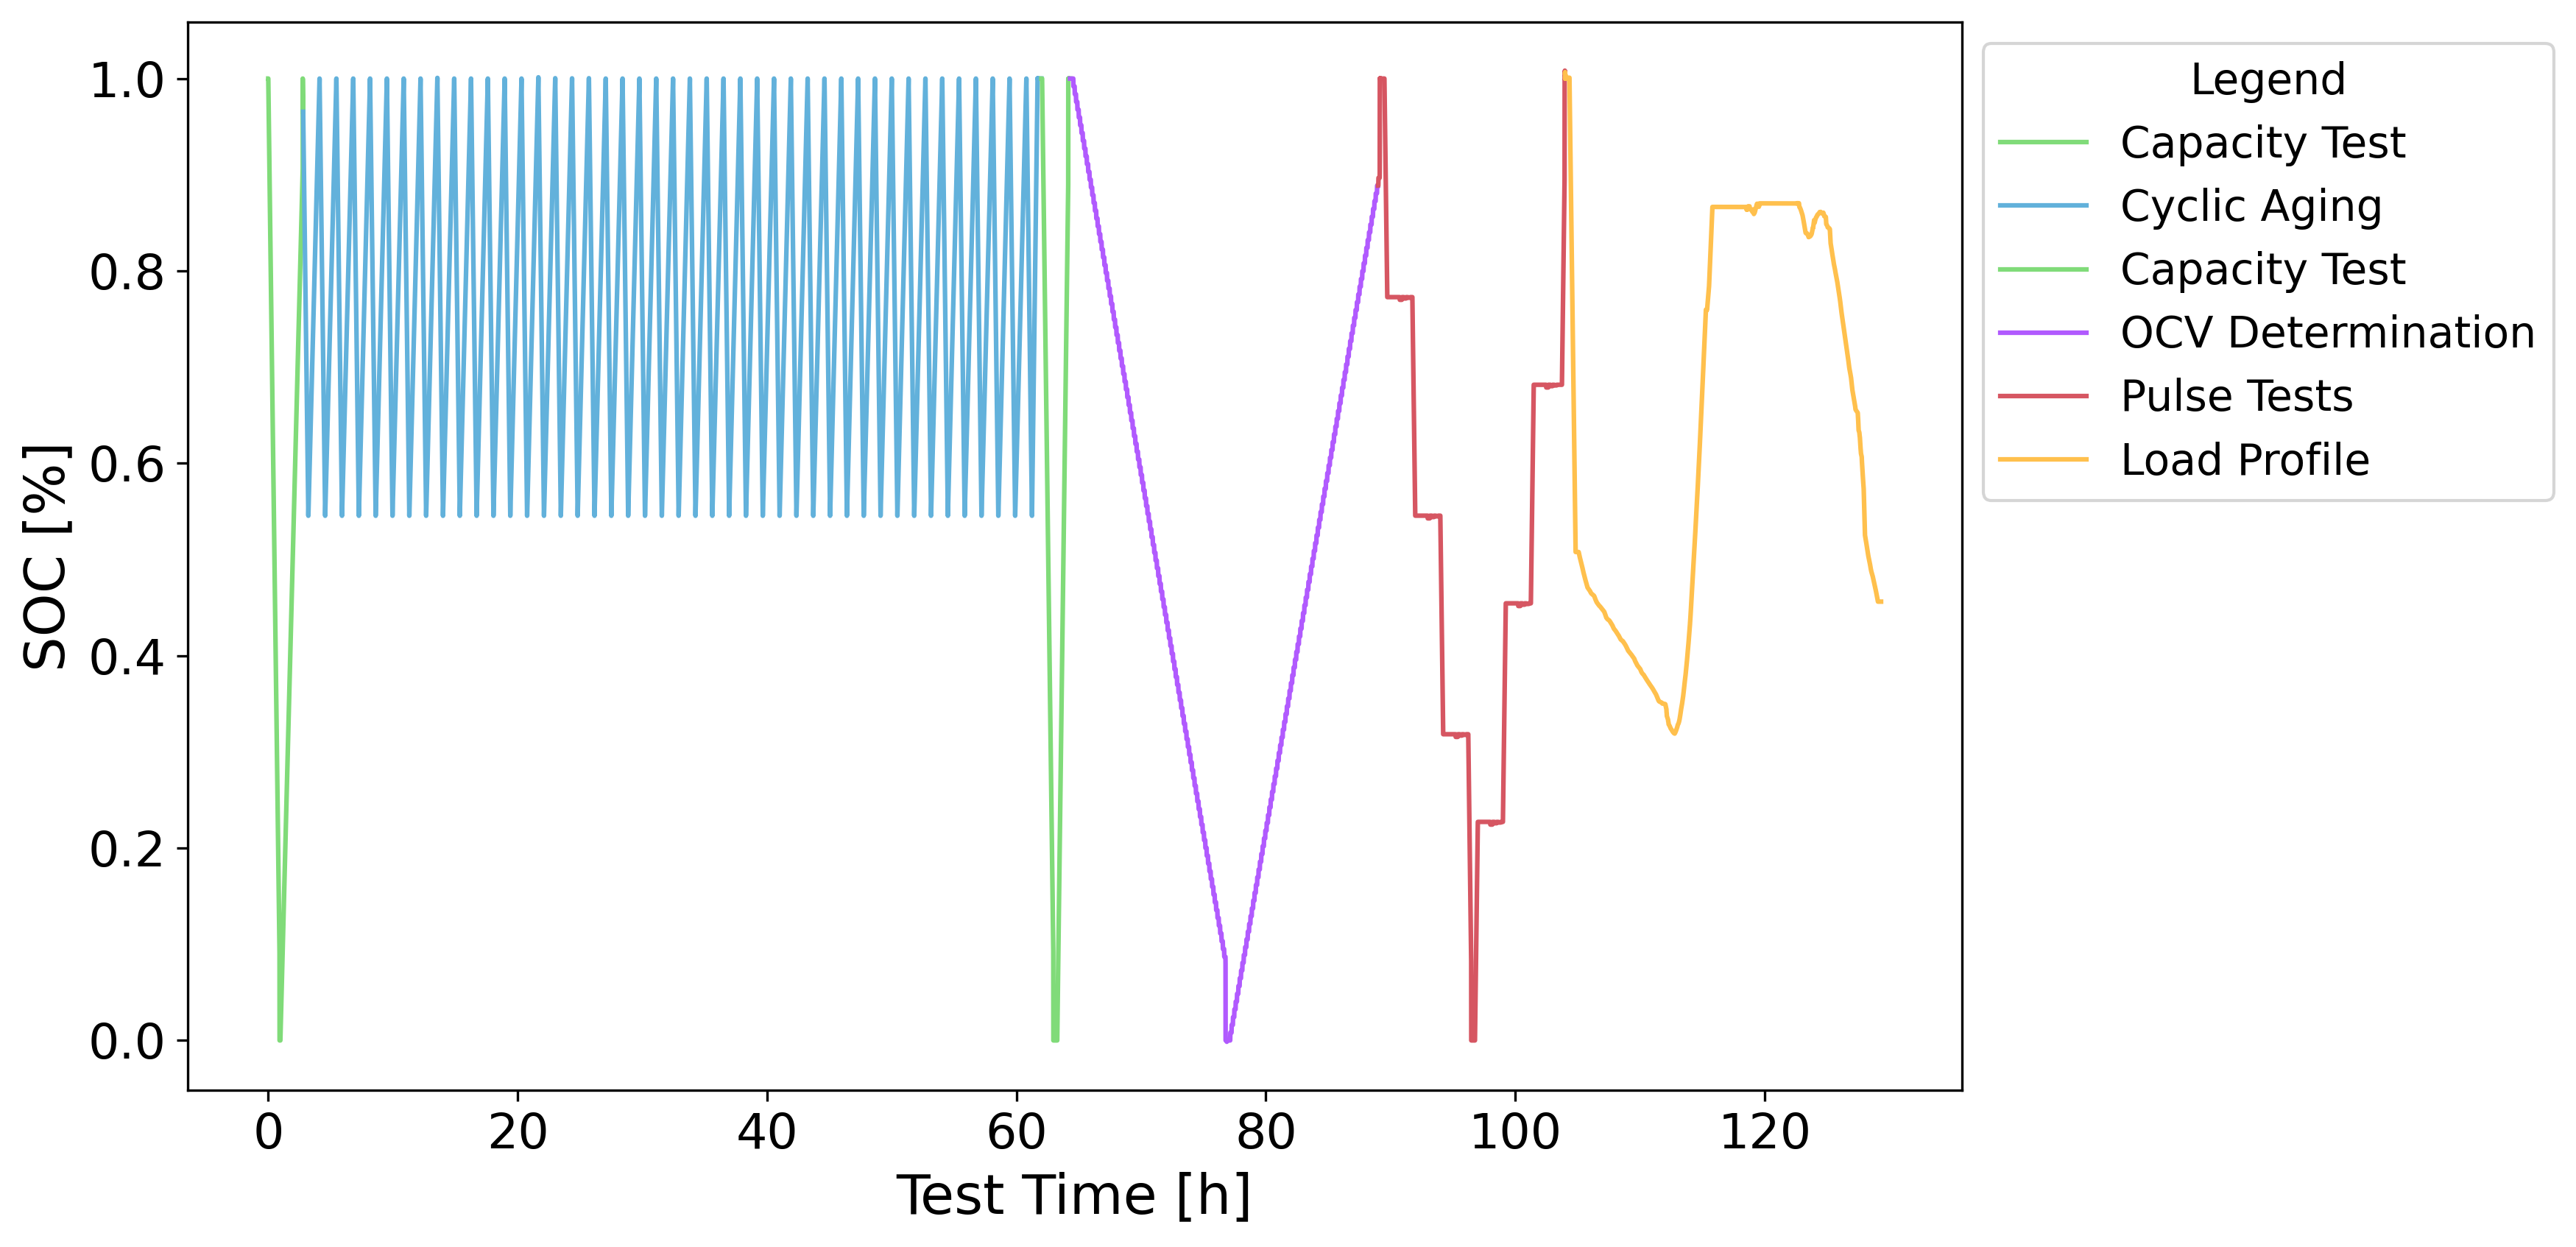
\includegraphics[width=\columnwidth]{figures/Combined_Results/Figure_3_SOC_Test_Trajectory.png}
    \caption[Representative SOC trajectory]{Representative SOC trajectory illustrating selected segments of the experimental protocol used in this study. The plot shows a portion of the cyclic ageing procedure with defined charge and discharge currents and a specified depth-of-discharge (DoD), followed by the diagnostic checkup sequence comprising OCV determination, HPPC pulses, and capacity tests. In addition, the trajectory includes a load profile taken from a stationary battery storage system. Together, these segments capture both controlled laboratory diagnostics and application-oriented operating conditions.}
    \label{fig:soc_tests}
\end{figure}
\begin{figure}[htbp]
    \centering
    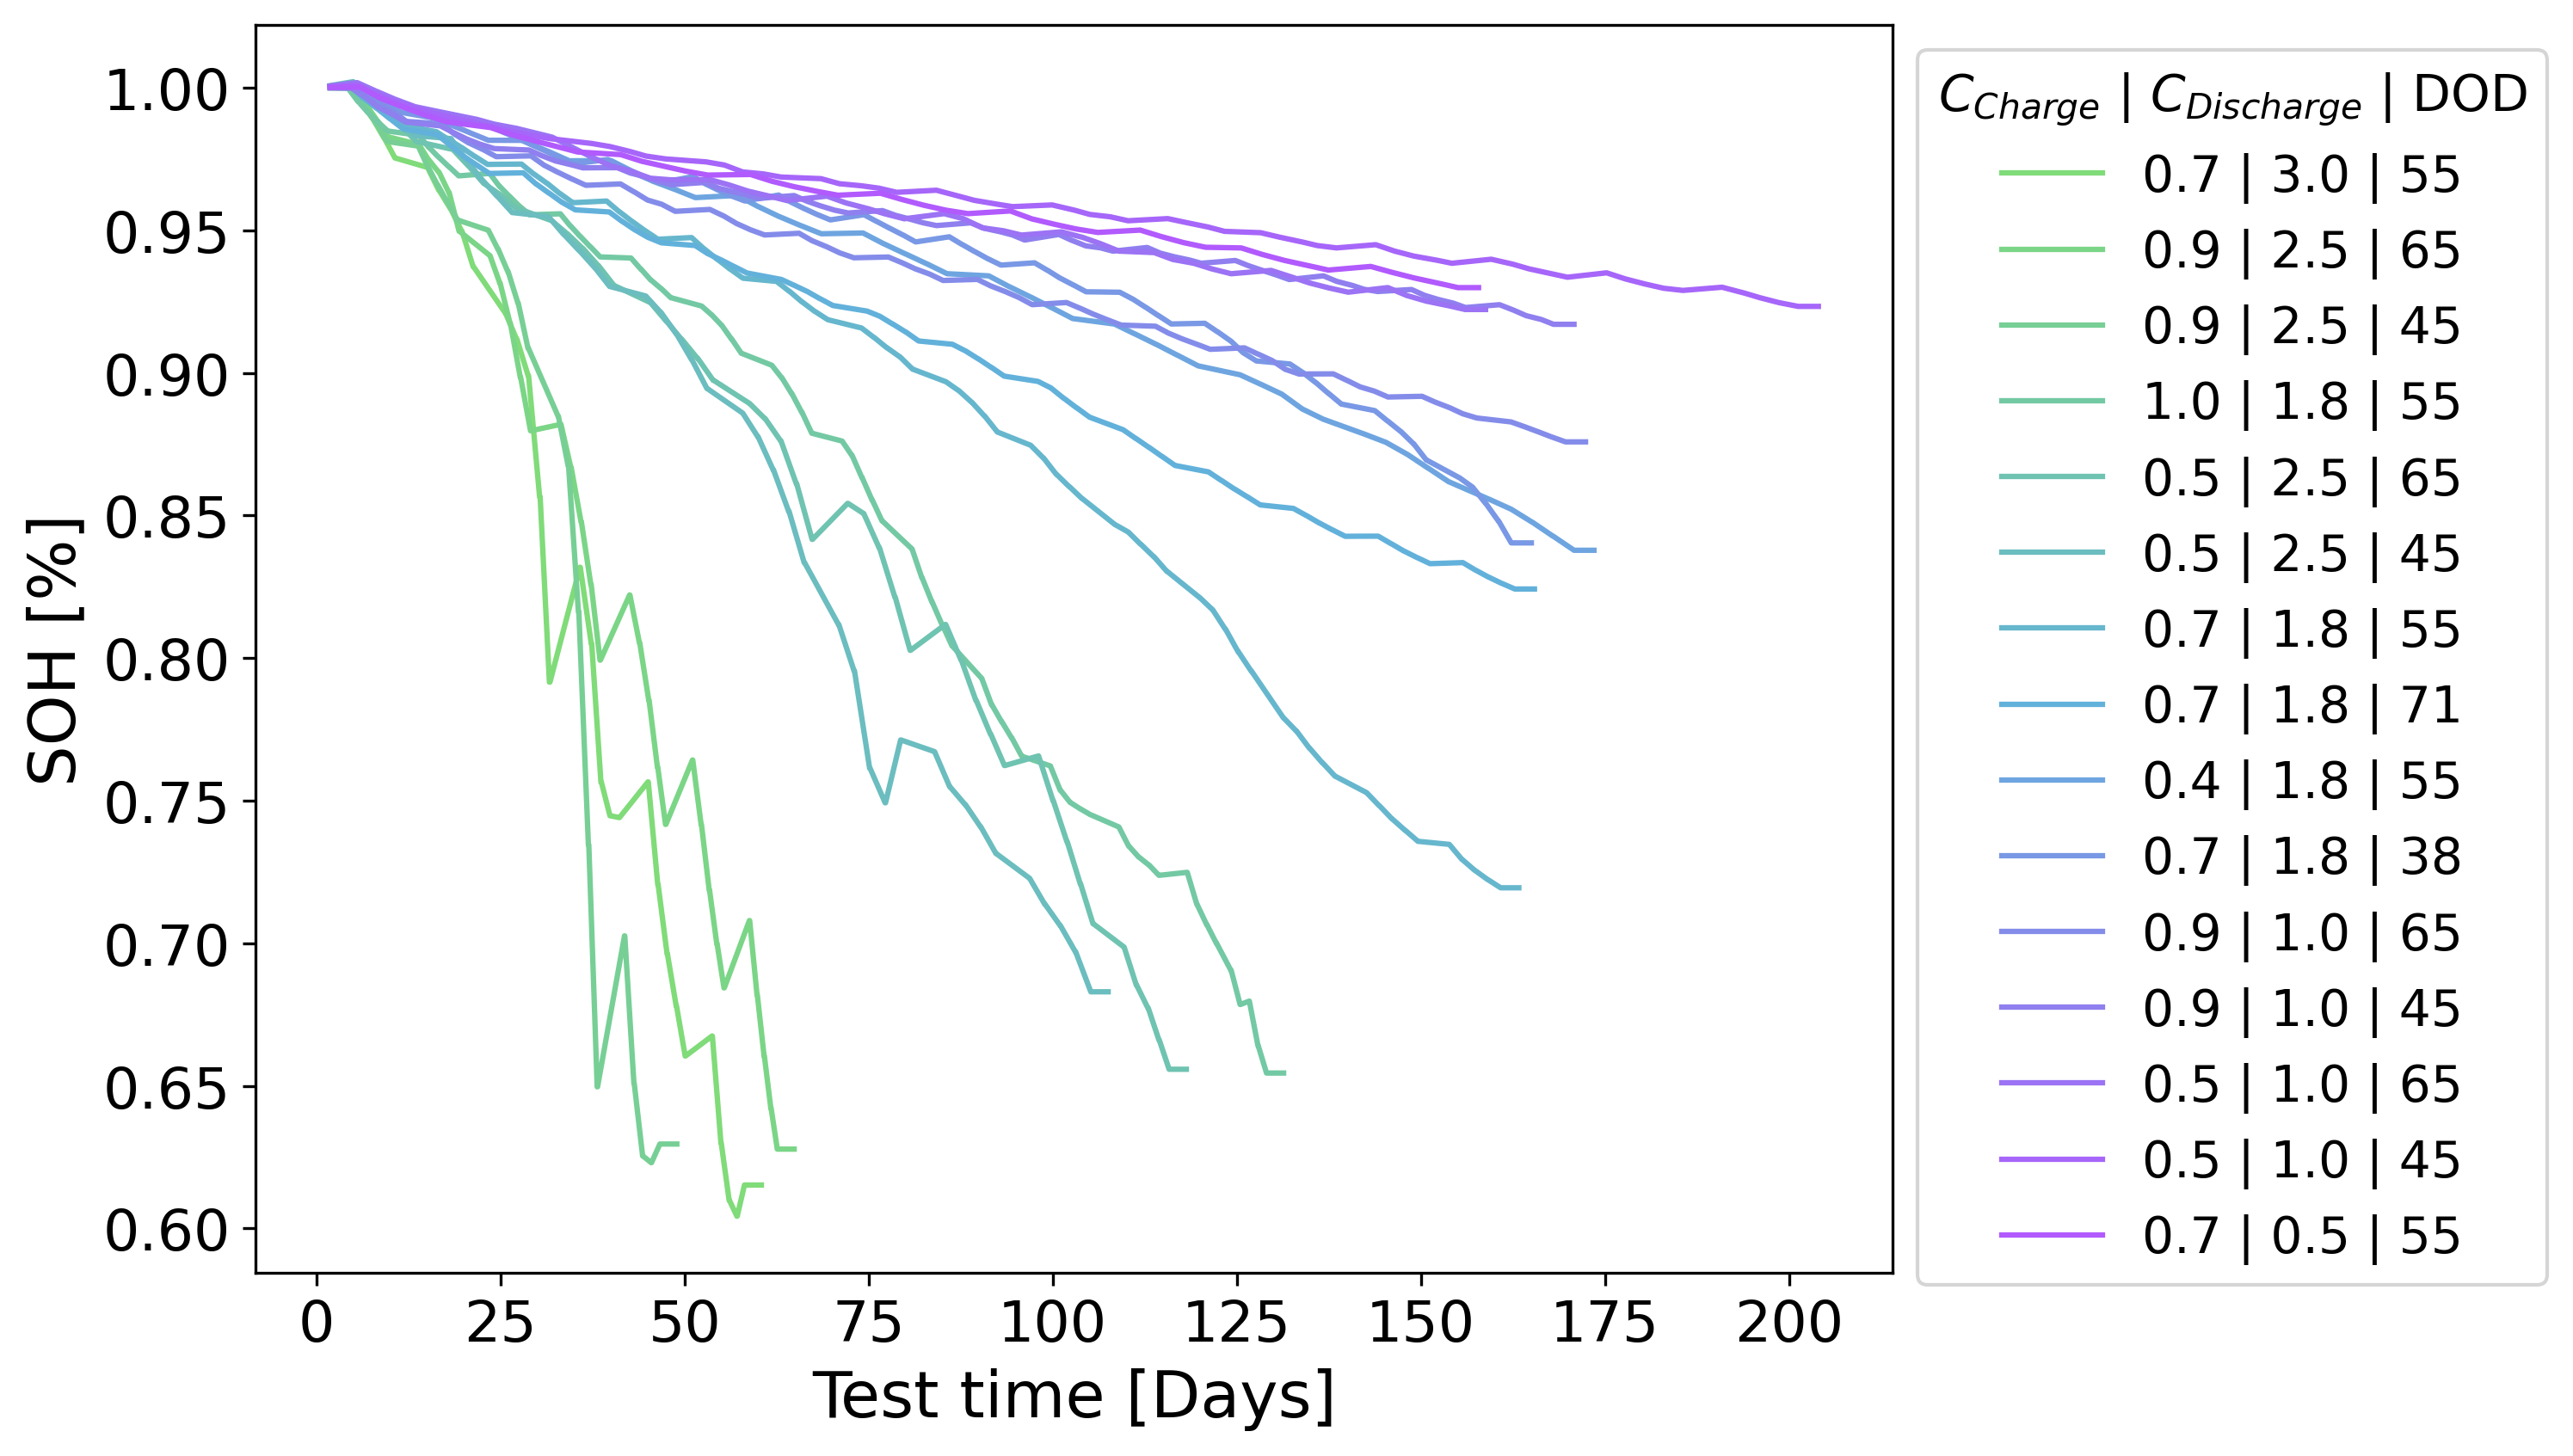
\includegraphics[width=\columnwidth]{figures/Combined_Results/Figure_4_SOH_All_Days.png}
    \caption[SOH across all cells]{Evolution of the state of health across all LFP cells in the ageing campaign, shown over the total experimental duration. The spread between trajectories reflects the different operating points in the factorial plan (C-rates, depth of discharge, profile mix) and motivates the use of a data-driven SOH estimator that generalises across cells and loading conditions.}
    \label{fig:soh_all_days}
\end{figure}
\noindent
Together, Figures~\ref{fig:soc_tests} and~\ref{fig:soh_all_days} illustrate the diversity of SOC transients and ageing behaviour that the estimators must capture: short-term SOC dynamics are driven by fast current swings and mode changes between profiles, whereas SOH evolves slowly over hundreds of days and depends on the cumulative operating conditions of each cell.
\subsection{Feature Engineering}
The SOC model consumes the six-dimensional feature vector
\begin{equation}
    \mathbf{x}^{\mathrm{SOC}}_t = \bigl[U(t),\, I(t),\, T(t),\, Q_c(t),\, \tfrac{\mathrm{d}U}{\mathrm{d}t}(t),\, \tfrac{\mathrm{d}I}{\mathrm{d}t}(t)\bigr],
\end{equation}
where temporal derivatives are obtained via centred finite differences. Each component is normalised using a robust scaling operation based on the median $m$ and interquartile range $r$: 
\begin{equation}
    \tilde{x}^{\mathrm{SOC}}_{t,k} = \frac{x^{\mathrm{SOC}}_{t,k} - m_k}{r_k + \varepsilon}, \qquad \varepsilon=10^{-6}.
\end{equation}
The same $(m_k,r_k)$ pairs are embedded in the firmware so that the STM32 receives identically normalised inputs. 
The SOH model uses a slightly different feature stack to capture slow-varying degradation markers:
\begin{equation}
    \mathbf{x}^{\mathrm{SOH}}_t = \bigl[ t,\, U(t),\, I(t),\, T(t),\, \mathrm{EFC}(t),\, Q_c(t) \bigr],
\end{equation}
where $t$ is the cumulative time stamp and $\mathrm{EFC}(t)$ denotes the equivalent full cycles accrued up to sample $t$. These channels are likewise robustly normalised, relying on median and interquartile range rather than mean and variance to reduce the influence of outliers in current and voltage measurements~\cite{huberRobustStatistics2009,pedregosaScikitlearnMachineLearning2012}. During deployment the SOC and SOH models run independently on the microcontroller: the SOC and SOH model provides a high-rate estimate at 1~Hz. In principle both estimates could be fused more tightly, but in this work we keep the models separate in order to study their resource usage and accuracy in isolation.
\subsection{Reference SOC and SOH targets}
The ground-truth SOC trajectory is derived from Coulomb counting with drift compensation. Denoting the apparent cell capacity after a given check-up by $C_{\mathrm{app}}$, the SOC inside a charge-discharge segment is computed as
\begin{equation}
    \mathrm{SOC}(t) = \mathrm{SOC}(t_0) - \frac{1}{C_{\mathrm{app}}}\int_{t_0}^{t} I(\tau)\,\mathrm{d}\tau,
\end{equation}
where the integral is reset to $\mathrm{SOC}=1$ after each constant-voltage (CV) termination. The reset mitigates the bias that would otherwise accumulate due to capacity fade, yet the long-term traces still reveal gradual changes in the SOC envelope as $C_{\mathrm{app}}$ decreases.
State of health is obtained from the periodic capacity check-ups through
\begin{equation}
    \mathrm{SOH}_k = \frac{C_k}{C_{\mathrm{nom}}},
\end{equation}
with $C_k$ representing the measured discharge capacity during the $k$-th reference cycle (comprising capacity test, open-circuit-voltage sweep, and hybrid pulse-power characterisation) relative to the nominal capacity $C_{\mathrm{nom}}$. These targets highlight the need for a data-driven estimator that remains accurate despite the evolving capacity landscape, which motivates the use of recurrent neural networks for both SOC and SOH predictions.
The reference SOC and SOH traces are therefore offline constructs. They rely on information that is not available in deployment, such as long rest periods for OCV stabilisation and capacity from periodic full cycles, and they assume perfect initialisation and recalibration. These constructions follow common practice in battery management, where SOC is obtained by Coulomb counting and SOH is expressed as the ratio between present and nominal capacity~\cite{plettBatteryManagementSystems2015,a.m.s.m.h.s.attanayakaEstimationStateCharge2019,berecibarCriticalReviewState2016}. On the STM32 the estimators operate purely on the streamed measurements and their internal states; the reference trajectories only serve as ground truth for training and evaluation.
\subsection{Streaming inference setup}
Because the SOC and SOH estimators are stateful, the LSTM hidden and cell states are continuously forwarded from one sample to the next along the full input stream. At each sampling instant the current feature vector is processed together with the previous hidden and cell states, which yields the new states and the corresponding SOC or SOH estimate. We therefore operate the models in a purely step-by-step streaming regime without forming sliding input windows. On the host the full normalised sequence from the LFP DoE Cycle Ageing Dataset is processed once in this fashion, and the resulting SOC and SOH estimates are aligned with the reference trajectories. On the STM32 firmware the same step-wise LSTM implementation is used, driven by the UART feature stream, so that host and embedded benchmarks reflect identical inference conditions. The streaming dashboards in Figs.~\ref{fig:soc_dashboard} and~\ref{fig:soh_dashboard} illustrate a complete run for one representative cell.
\section{Model Architecture and Baseline Performance}
\subsection{LSTM architecture in PyTorch}
Both SOC and SOH estimators employ the same recurrent equation set but differ in size according to their training releases. The SOC configuration uses $H=64$ hidden units and an MLP output layer of width~64, whereas the SOH configuration increases both dimensions to~128 to cope with the longer temporal context. LSTM gates $i_t,f_t,o_t$ and candidate state $g_t$ follow the standard formulation used in modern RNN surveys~\cite{liptonCriticalReviewRecurrent2015}. All models are implemented in PyTorch~\cite{paszkePyTorchImperativeStyle2019}.
\begin{align}
    \mathbf{z}_t &= [\mathbf{x}_t,\mathbf{h}_{t-1}],\\
    \mathbf{i}_t &= \sigma(W_i \mathbf{z}_t + \mathbf{b}_i), \quad
    \mathbf{f}_t = \sigma(W_f \mathbf{z}_t + \mathbf{b}_f), \nonumber\\
    \mathbf{o}_t &= \sigma(W_o \mathbf{z}_t + \mathbf{b}_o), \quad
    \mathbf{g}_t = \tanh(W_g \mathbf{z}_t + \mathbf{b}_g), \nonumber\\
    \mathbf{c}_t &= \mathbf{f}_t \odot \mathbf{c}_{t-1} + \mathbf{i}_t \odot \mathbf{g}_t,\quad
    \mathbf{h}_t = \mathbf{o}_t \odot \tanh(\mathbf{c}_t). \nonumber
\end{align}
Both SOC and SOH models are trained with a mean-squared-error loss between the prediction and the corresponding reference at each training sample. During validation we additionally report mean absolute error (MAE), root-mean-square error (RMSE), and $R^2$. The trained parameters, together with the corresponding configuration files and optimiser statistics, are archived to enable deterministic replays of both models.
\subsection{Training Notes}
Training is carried out on a GPU node equipped with NVIDIA A100-class accelerators using mixed-precision (FP16) arithmetic. Both SOC and SOH models use the AdamW optimiser with cosine-annealing warm-restart scheduling, gradient clipping, and mini-batch training~\cite{loshchilovDecoupledWeightDecay2017,loshchilovSGDRStochasticGradient2016,micikeviciusMixedPrecisionTraining2017,pascanuDifficultyTrainingRecurrent2012}. For SOC we use a learning rate of $1.5\times10^{-4}$, a batch size of~512, and sequence chunks of length~2024, whereas SOH training employs a learning rate of $2.0\times10^{-4}$, a batch size of~128, and chunks of length~2048 with otherwise identical optimisation settings. Although deployment operates the LSTM in fully stateful, step-by-step streaming mode, training thus relies on truncated backpropagation through time over these windows. Within each chunk the hidden and cell states are propagated across time exactly as in deployment, so the stateful update mechanism is already learned during training, while the windowing allows randomised sampling of sequence segments, accelerates convergence, and improves generalisation across the diverse ageing trajectories.
\subsection{Baseline Accuracy}
On the workstation the SOC and SOH base models are first evaluated in streaming mode on the full ageing trajectory of one representative LFP cell from the LFP DoE Cycle Ageing Dataset~\cite{LFP_DoE_Cycle_Aging_Dataset}, yielding baseline MAE and RMSE values for both tasks. These Python replays operate on the original PyTorch implementations and serve as a numerical reference for all subsequent experiments. The same checkpoints are then pruned, quantized, and exported to STM32 firmware, where identical feature streams are replayed to measure not only accuracy but also flash and RAM usage, system latency, on-device inference time, and energy per inference (cf. Section~\ref{sec:kpis}). Figure~\ref{fig:pipeline} summarises this training-to-firmware benchmarking pipeline.
\begin{figure*}[t!]
    \centering
    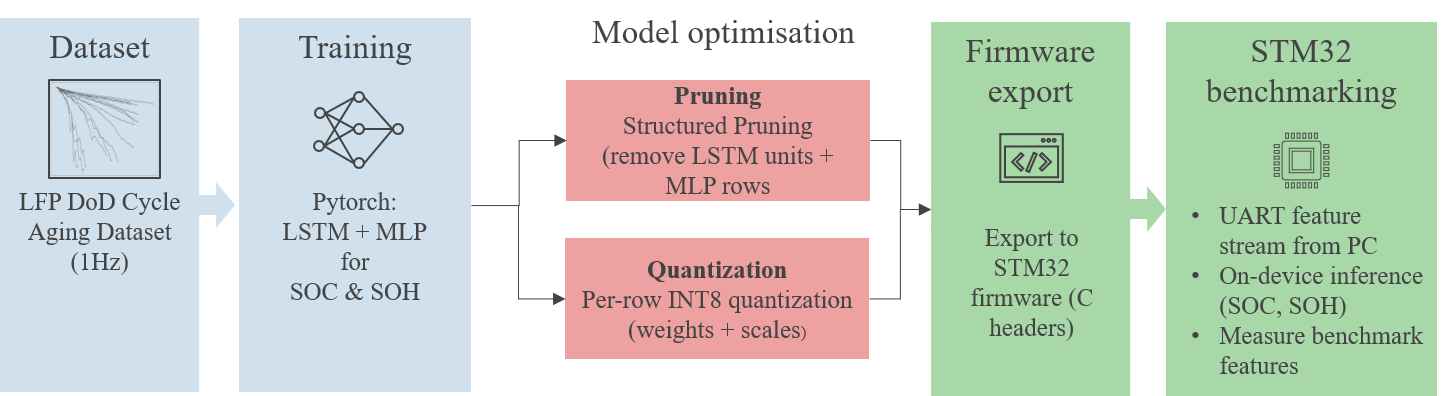
\includegraphics[width=\textwidth]{figures/Schematics/Figure_5_Pipeline.png}
    \caption[End-to-end pipeline]{End-to-end pipeline from dataset to embedded benchmarking. The LFP DoE Cycle Ageing Dataset feeds PyTorch training on a GPU workstation; the resulting SOC and SOH LSTM\,+\,MLP models are pruned and quantized, exported as C headers, and deployed on an STM32H753ZI board, where flash/RAM usage, inference time, latency, and energy are measured under streaming replay.}
    \label{fig:pipeline}
\end{figure*}
\section{Pruning}
Pruning reduces the size and computational cost of a neural network by eliminating parameters or whole units that contribute little to the overall mapping, while keeping the input-output behaviour as close as possible to the dense baseline~\cite{hanLearningBothWeights2015,blalockWhatStateNeural2020}. In our setting we apply structured pruning at the level of complete LSTM hidden units so that the resulting model remains well suited for efficient C implementations on the microcontroller.
\subsection{Structured magnitude pruning}
Structured magnitude pruning removes the lowest-saliency LSTM units until only $45$ hidden channels remain in the SOC model (30\% sparsity), with analogous settings for the SOH experiments. Reducing the state dimension is a prerequisite for fitting the estimators into the flash and SRAM budgets of the target STM32-based BMS and for shortening the on-device inference time, inspired by structured sparsity approaches for deep and recurrent networks~\cite{wenLearningStructuredSparsity2016,lobachevaStructuredSparsificationGated2020,narangExploringSparsityRecurrent2017}. In analogy to the group-lasso style regularisers proposed for LSTMs in~\cite{wenLearningStructuredSparsity2016,lobachevaStructuredSparsificationGated2020}, which aggregate weights across gates via L2 norms, we define a saliency score for each hidden unit $h$ that combines all incoming weights from the different gates:
\begin{equation}
    s_h = \sum_{g\in\{i,f,o,g\}} \left(\lVert W_{\mathrm{ih}}^{(g)}[h,:]\rVert_2 + \lVert W_{\mathrm{hh}}^{(g)}[h,:]\rVert_2\right).
\end{equation}
Units are ranked by $s_h$ and the top $H'$ indices are retained. In the final deployments we use $H'=45$ hidden units for the SOC estimator and $H'=90$ units for the SOH estimator, corresponding to roughly 30~\% channel-wise sparsity with respect to the original architectures. Pruned rows and columns are removed jointly from all gate matrices as well as from the downstream MLP weights, ensuring that the reduced network still implements a valid recurrent mapping. After each pruning step the network is fine-tuned on the training data before the next pruning round commences.
\begin{figure}[t]
    \centering
    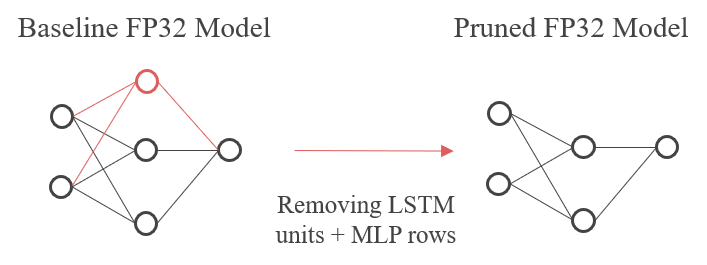
\includegraphics[width=\columnwidth]{figures/Schematics/Figure_6_Pruning_Schematic.png}
    \caption{Schematic illustration of structured pruning. The left panel highlights a low-saliency hidden unit and its incident connections in red, while the right panel shows the resulting network after removing the corresponding unit and weights. In the SOC/SOH architecture this procedure is applied at the level of complete LSTM hidden channels and the associated MLP rows.}
    \label{fig:pruning_schematic}
\end{figure}
\subsection{Resulting pruned models}
The resulting pruned SOC and SOH models still run in FP32 but reduce flash consumption and runtime considerably once compiled for STM32. Section~\ref{sec:kpis} summarises the corresponding latency and memory savings. These pruned variants are evaluated alongside their base and quantized counterparts throughout the results section.
\section{Quantization}
Quantization complements pruning by reducing the numerical precision of the remaining weights while keeping the network topology unchanged. In this work we apply post-training quantization to the SOC and SOH LSTM\,+\,MLP models so that the recurrent weights are stored as 8-bit integers with associated floating-point scales, enabling compact storage and efficient integer arithmetic on the microcontroller. An 8-bit integer can encode $2^8 = 256$ distinct levels; a signed int8 representation uses the code book $\{-128,\ldots,127\}$ so that positive and negative weights share a symmetric dynamic range around zero. An unsigned mapping $\{0,\ldots,255\}$ would instead centre the quantizer around $127.5$ and treat negative values asymmetrically, which is undesirable for zero-centred weight distributions. The factor $127$ in the scale definition below therefore ensures that the largest-magnitude weight in a row maps close to $\pm 127$ while keeping zero exactly representable, following standard uniform int8 post-training quantization schemes~\cite{jacobQuantizationTrainingNeural2017,krishnamoorthiQuantizingDeepConvolutional2018}. Conceptually, each FP32 weight $w$ is then mapped to an integer $q$ by a scalar quantizer and reconstructed approximately as
\begin{align}
    q &= \mathcal{Q}_s(w), \label{eq:int8_q}\\
    \hat{w} &= s\,q, \label{eq:int8_w}
\end{align}
where $s>0$ denotes a scale factor and $\mathcal{Q}_s : \mathbb{R} \rightarrow \{-128,\ldots,127\}$ is a uniform mid-tread quantizer that rounds $w/s$ to the nearest integer and saturates the result to the closed interval $[-128,127]$ whenever necessary.
\subsection{Quantization Method}
In practice a per-row scale $s$ is chosen such that the maximum absolute weight in a row vector $w^{(r)} = (w_h)_h$ of a weight matrix $W$ (either $W_{\mathrm{ih}}$ or $W_{\mathrm{hh}}$) maps close to the int8 limits, for example
\begin{equation}
    s = \frac{\max_h |w_h|}{127},
\end{equation}
and all weights in that row are quantized according to~\eqref{eq:int8_q}. The resulting integer weights and their FP32 scales are then consumed by the gate computation in~\eqref{eq:quant}, while biases and activations remain in floating point.
\subsection{Quantization Details}
Per-row symmetric quantization is used for $W_{\mathrm{ih}}$ and $W_{\mathrm{hh}}$ so that each gate row receives its own floating scaling factor. Here $x$ denotes the current input feature vector, $h$ the previous hidden state, $W_{\mathrm{ih}}^{\mathrm{int8}}$ and $W_{\mathrm{hh}}^{\mathrm{int8}}$ the quantized input-to-gate and hidden-to-gate weight matrices, $s_{\mathrm{ih}}$ and $s_{\mathrm{hh}}$ the corresponding per-row scale vectors, and $b_{\mathrm{fp32}}$ the FP32 bias of the considered gate. Biases and activations remain FP32, ensuring that the STM32 implementation reproduces the PyTorch activations gate by gate. A built-in streaming comparison validates the conversion and typically yields MAE differences below $10^{-4}$. The gate computation used in firmware is
\begin{equation}
\label{eq:quant}
g = (xW_{\mathrm{ih}}^{\mathrm{int8}}) \cdot s_{\mathrm{ih}} + (hW_{\mathrm{hh}}^{\mathrm{int8}})\cdot s_{\mathrm{hh}} + b_{\mathrm{fp32}}.
\end{equation}
The INT8 representation reduces the recurrent weight memory footprint by roughly a factor of four compared with FP32 storage, which substantially eases the memory pressure when hosting the estimators on the STM32H753ZI MCU of the in-house BMS.
\begin{figure*}[t!]
    \centering
    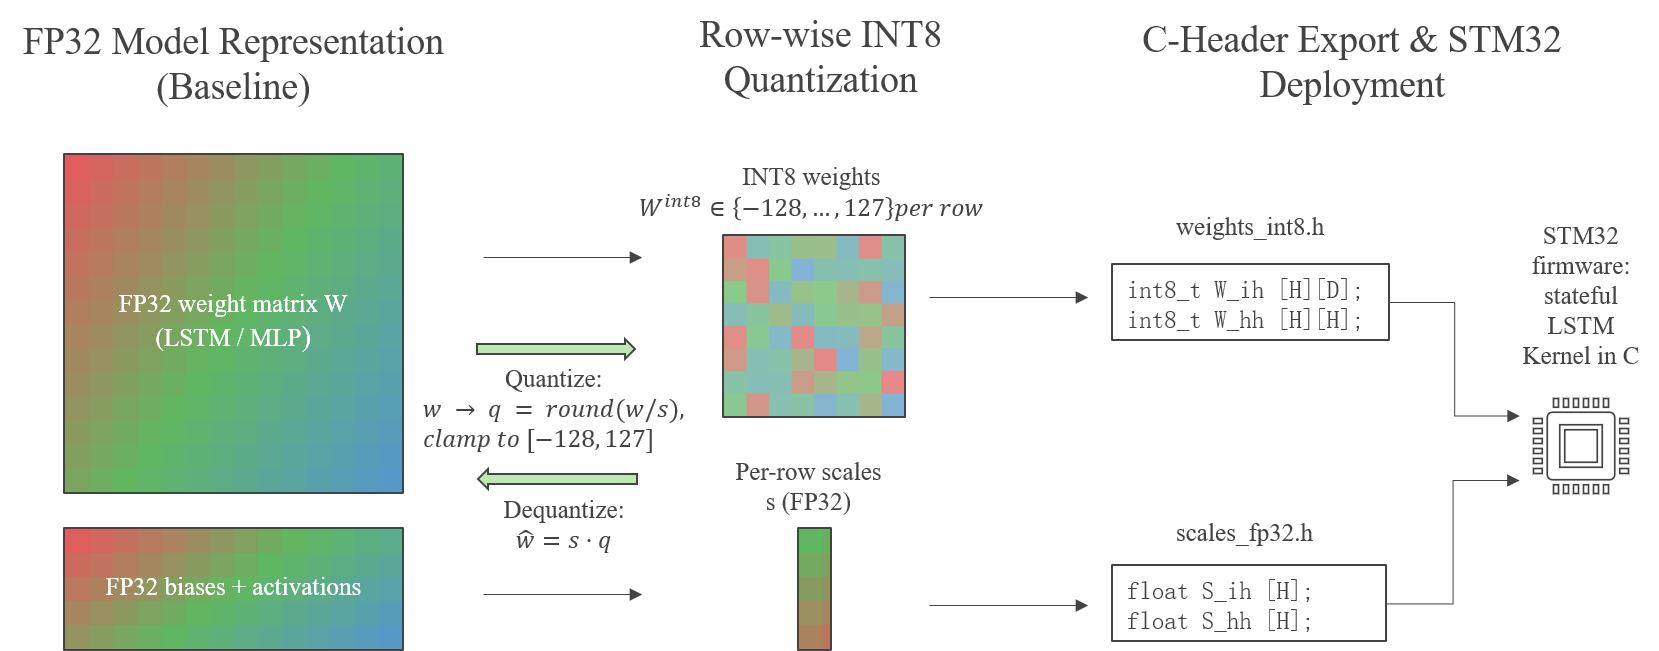
\includegraphics[width=\textwidth]{figures/Schematics/Figure_7_Quantization_Schematic.png}
    \caption{Illustration of the FP32-to-INT8 quantization scheme and embedded deployment. The left panel shows the baseline FP32 weight matrix and FP32 biases/activations. In the centre, per-row symmetric uniform quantization maps each row to an INT8 codebook $\{-128,\ldots,127\}$ together with a floating-point scale, following~\eqref{eq:int8_q}--\eqref{eq:quant}. The resulting integer weights and scale vectors are exported as C headers and consumed by the stateful LSTM kernel on the STM32H753ZI, which reconstructs the effective weights during on-device inference.}
    \label{fig:quantization_schematic}
\end{figure*}
\subsection{Export for STM32}
The exported headers integrate into the STM32 firmware project, which implements separate stateful LSTM\,+\,MLP models for SOC and for SOH as well as UART-based telemetry in~C. A small driver library provides build files and flashing scripts so that identical measurement binaries can be rebuilt on other machines. This explicit tool chain, from training through pruning and quantization to firmware, avoids hidden compiler optimisations and makes the resource measurements in Section~\ref{sec:kpis} reproducible.
\section{Benchmark Methodology}\label{sec:kpis}
This section describes how we benchmark the SOC and SOH models on both the host PC and an STM32 Nucleo-144 development board with an STM32H753ZI MCU~\cite{STM32Nucleo144Boards2025_Datasheet,naguibMicroprocessorExecutionTime2022}. The microcontroller provides \SI{2}{\mega\byte} of on-chip Flash and \SI{1}{\mega\byte} of SRAM, which constitute the budget for firmware code, model parameters, and runtime buffers. Starting from the trained LSTM\,+\,MLP models, we generate three embedded variants (full-precision baseline, pruned model, and quantized model) and evaluate them on the \emph{LFP DoE Cycle Ageing Dataset}. The benchmark combines long-horizon streaming simulations with hardware-in-the-loop measurements and is fully scripted to ensure reproducible accuracy and resource evaluations.

On the host side, the complete reference ageing sequence is replayed in Python using the same streaming inference functions that are later exported to C. The SOC and SOH estimators are evaluated in continuous time without windowing, and error metrics (MAE, RMSE, $R^2$), error histograms, and parity plots are computed from the resulting trajectories. These simulations provide a high-precision reference for the embedded experiments and are used to assess how pruning and quantization affect the dynamics of the baseline models.

For the embedded benchmarks the base, pruned, and quantized SOC/SOH models are embedded into dedicated firmware projects for the STM32H753ZI. Because STM32Cube~AI does not natively support stateful LSTM layers, the recurrent update equations, post-processing, and UART diagnostics are implemented manually in C. Identical stimulus streams are then injected via UART, allowing a direct comparison between host-side and on-device behaviour under the same operating conditions.

\subsection{STM32 Measurements}
On the STM32 Nucleo-144 development board, dedicated SOC and SOH firmware images execute the embedded estimators while host-side scripts handle stimulus injection and UART logging. Recorded feature streams are pushed through the UART into the microcontroller, which runs the stateful LSTM\,+\,MLP in a tight loop and emits the corresponding SOC or SOH predictions together with timing diagnostics. Each sample produces two time stamps: a host-side latency in milliseconds that measures the delay between sending an input vector and receiving its estimate, and an on-device inference time in microseconds that reflects only the execution time of the core LSTM and MLP kernels on the STM32 (derived from the DWT cycle counter). The average on-device inference time, combined with an empirically calibrated average board power, yields the energy per inference reported in Section~\ref{sec:kpis}.

\subsection{Key Performance Indicators}
For each deployment we report embedded performance metrics in the form of average host latency, on-device inference time, memory usage (flash and SRAM for code, weights, and buffers), and energy per inference. The error metrics (MAE and RMSE) are analysed in the PC streaming section and in the corresponding histograms; Tables~\ref{tab:kpi} and~\ref{tab:kpi_soh} therefore focus on STM32 resource and timing indicators. In these tables the latency entry denotes the mean end-to-end delay between transmitting a feature vector over UART and receiving the corresponding SOC/SOH estimate on the host, whereas the inference time isolates the execution of the LSTM\,+\,MLP kernels on the microcontroller and is measured via the DWT cycle counter. The RAM figures are obtained by summing the statically allocated data (.data and .bss) with the maximum stack usage observed during streaming, converted to kilobytes, and the energy per inference is approximated by multiplying the average on-device inference time with an empirically calibrated average board power of \SI{0.5}{\watt}, yielding reproducible microjoule values without re-running the external power measurements.
For each deployment we report embedded performance metrics in the form of average host latency, on-device inference time, memory usage (flash and SRAM for code, weights, and buffers), and energy per inference. The error metrics (MAE and RMSE) are analysed in the PC streaming section and in the corresponding histograms; Tables~\ref{tab:kpi} and~\ref{tab:kpi_soh} therefore focus on STM32 resource and timing indicators. In these tables the latency entry denotes the mean end-to-end delay between transmitting a feature vector over UART and receiving the corresponding SOC/SOH estimate on the host, whereas the inference time isolates the execution of the LSTM\,+\,MLP kernels on the microcontroller and is measured via the DWT cycle counter. The RAM figures are obtained by summing the statically allocated data (.data and .bss) with the maximum stack usage observed during streaming, converted to kilobytes, and the energy per inference is approximated by multiplying the average on-device inference time with an empirically calibrated average board power of \SI{0.5}{\watt}, yielding reproducible millijoule values without re-running the external power measurements.
\begin{table*}[t!]
      \centering
      \caption{Engineering KPIs for SOC models on STM32H753ZI (full-stream averages).}
      \label{tab:kpi}
        \begin{tabular}{lccccc}
            \toprule
            Model & Latency [ms] & Inference [ms] & Flash [KB] & RAM [KB] & Energy [mJ] \\
            \midrule
            Base FP32 & 12.70 & 1.40 & 105.32 & 4.93 & 0.70 \\
            Pruned FP32 & 12.20~\textcolor{mgGreen}{(-3.9\%)} & 0.80~\textcolor{mgGreen}{(-42.9\%)} & 62.27~\textcolor{mgGreen}{(-40.9\%)} & 4.03~\textcolor{mgGreen}{(-18.3\%)} & 0.40~\textcolor{mgGreen}{(-42.9\%)} \\
            Quant INT8 & 18.48~\textcolor{mgRed}{(+45.5\%)} & 6.99~\textcolor{mgRed}{(+399\%)} & 52.48~\textcolor{mgGreen}{(-50.2\%)} & 3.96~\textcolor{mgGreen}{(-19.7\%)} & 3.49~\textcolor{mgRed}{(+399\%)} \\
            \bottomrule
        \end{tabular}
  \end{table*}
An analogous set of measurements was recorded for the SOH firmware deployments. Table~\ref{tab:kpi_soh} lists the corresponding indicators.
  \begin{table*}[t!]
      \centering
      \caption{Engineering KPIs for SOH models on STM32H753ZI (full-stream averages).}
      \label{tab:kpi_soh}
        \begin{tabular}{lccccc}
            \toprule
            Model & Latency [ms] & Inference [ms] & Flash [KB] & RAM [KB] & Energy [mJ] \\
            \midrule
            Base FP32 & 34.88 & 22.73 & 335.00 & 8.69 & 11.37 \\
            Pruned FP32 & 24.69~\textcolor{mgGreen}{(-29.2\%)} & 12.72~\textcolor{mgGreen}{(-44.0\%)} & 182.41~\textcolor{mgGreen}{(-45.5\%)} & 6.96~\textcolor{mgGreen}{(-19.9\%)} & 6.36~\textcolor{mgGreen}{(-44.0\%)} \\
            Quant INT8 & 41.23~\textcolor{mgRed}{(+18.2\%)} & 29.21~\textcolor{mgRed}{(+28.5\%)} & 138.00~\textcolor{mgGreen}{(-58.8\%)} & 6.70~\textcolor{mgGreen}{(-22.9\%)} & 14.60~\textcolor{mgRed}{(+28.5\%)} \\
            \bottomrule
        \end{tabular}
\end{table*}

The KPIs in Tables~\ref{tab:kpi} and~\ref{tab:kpi_soh} highlight the trade-offs introduced by pruning and quantization.
For SOC, pruning reduces the flash footprint by roughly 41~\% and cuts both inference time and energy per inference
by about 43~\%, while keeping latency dominated by UART transfer. Quantization roughly halves the flash usage again,
but the additional de-quantization operations and integer--float conversions inside the hand-written kernels increase
the on-device inference time and energy by a factor of four compared with the dense baseline. The SOH deployments show
the same qualitative behaviour: pruning saves about 46~\% of flash and 44~\% of inference energy, whereas the
quantized variant attains the smallest flash footprint but incurs a moderate increase in computation time and energy.
These measurements demonstrate that pruning is the primary lever for improving energy efficiency on the STM32, while
quantization is most beneficial when non-volatile memory is the limiting resource.

\section{Results}
\label{sec:results}
In this section, we present a comprehensive evaluation of the proposed embedded AI pipeline. We analyse the performance of both the State-of-Charge (SOC) and State-of-Health (SOH) estimators, focusing on the trade-offs between the full-precision baseline, the pruned variant, and the quantized deployment. The results are derived from the continuous streaming replay of the high-resolution LFP DoE Cycle Ageing Dataset, ensuring that all transient effects and long-term drifts are captured.
\subsection{Streaming Prediction Accuracy}
The primary metric for any battery state estimator is its ability to track the ground truth over extended periods without divergence. Figures~\ref{fig:soc_dashboard} and~\ref{fig:soh_dashboard} illustrate the streaming performance of the SOC and SOH models over the complete test duration.
\begin{figure*}[tb]
    \centering
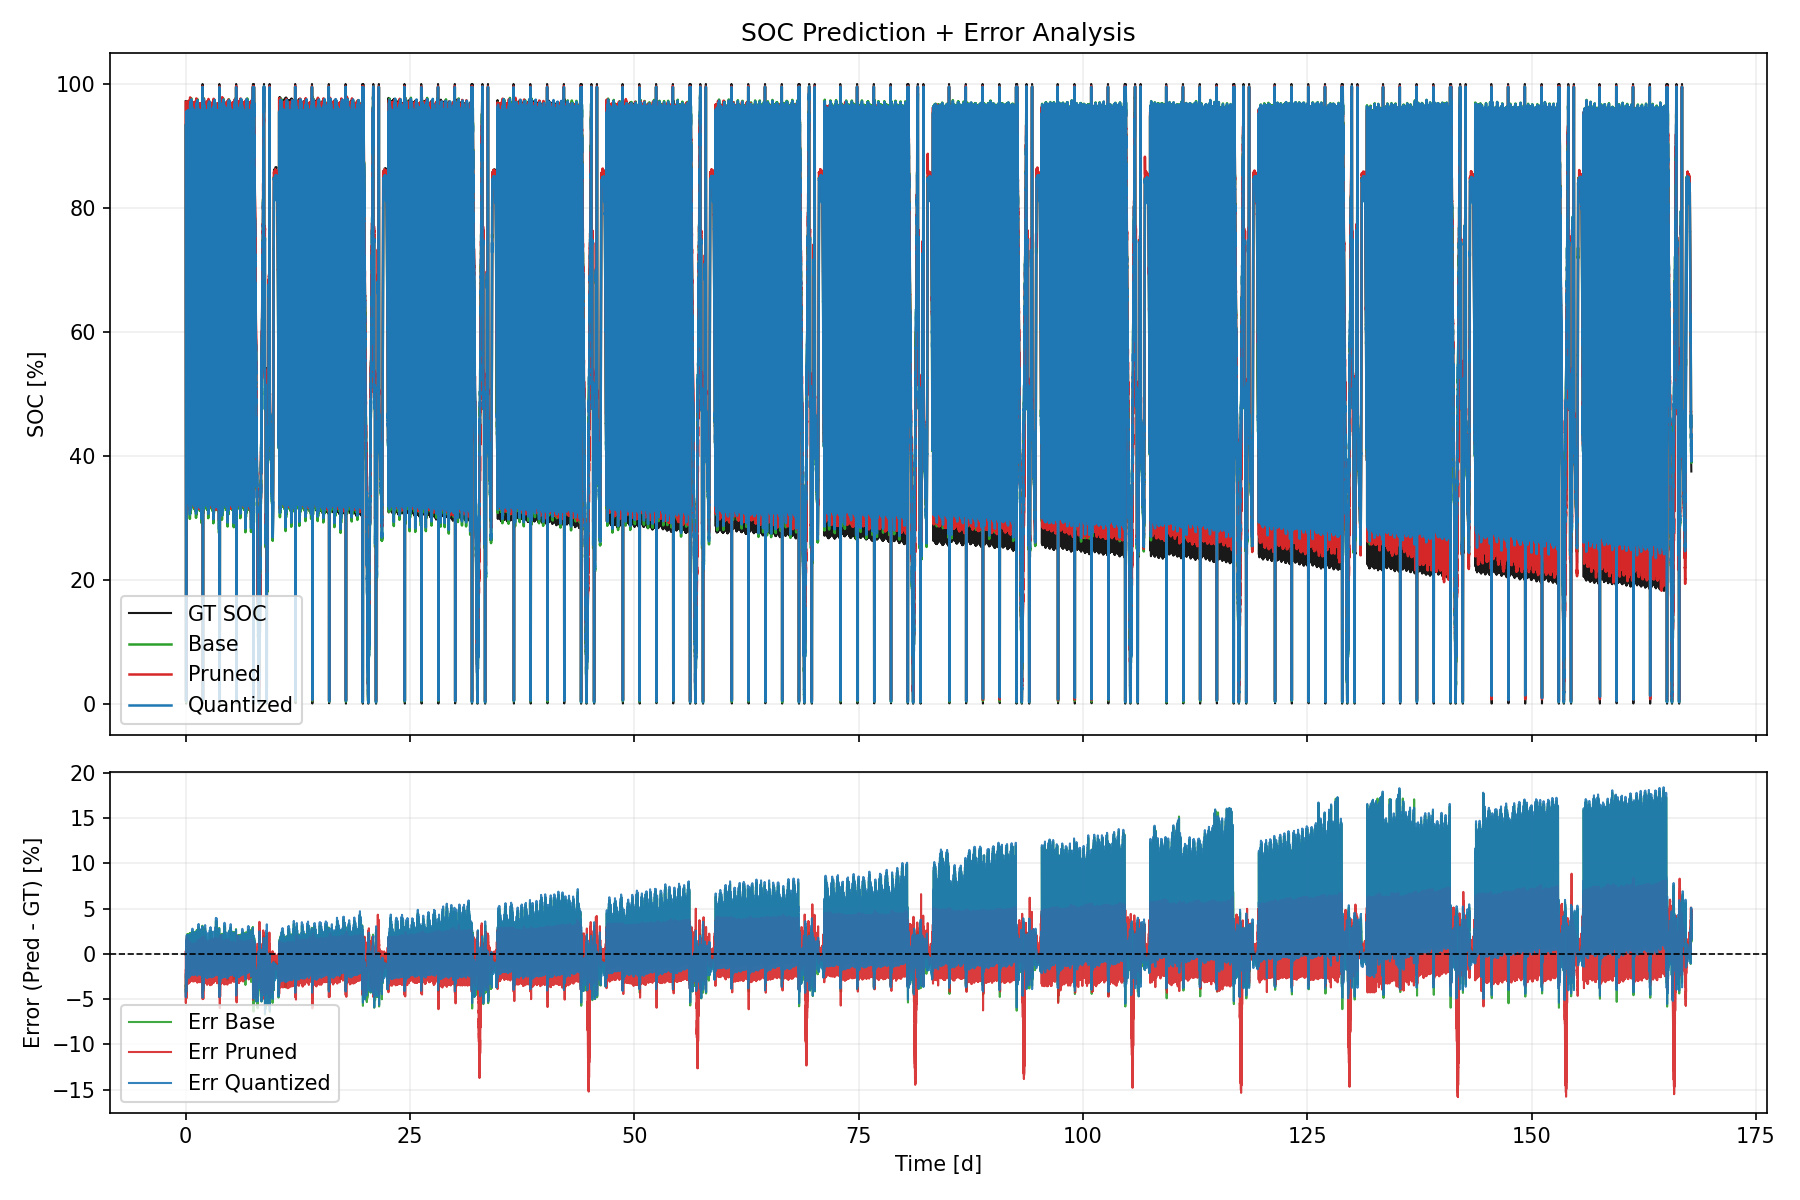
\includegraphics[width=\textwidth]{figures/Combined_Results/Figure_8_SOC_Streaming_Dashboard.png}
    \caption{Streaming SOC dashboard on the full ageing trajectory. The black line represents the reference SOC, while the coloured lines show the predictions of the Base (green), Pruned (red), and Quantized (blue) models. The lower sub-panel displays the instantaneous prediction error.}
    \label{fig:soc_dashboard}
\end{figure*}
For the SOC estimator, the tracking is exceptionally tight across the entire dynamic range. The error residuals remain centered around zero, with only minor excursions during extreme current steps. Notably, the quantized model (blue trace) overlaps the full-precision baseline (green trace) so closely that they are often visually indistinguishable. This confirms that our layer-wise symmetric quantization strategy preserves the recurrent dynamics essential for accurate Coulomb counting and voltage relaxation modelling. The pruned model (red trace), while still highly accurate, exhibits slightly larger deviations in highly dynamic regions, a simplified behaviour expected from the significant reduction in hidden state dimensionality.
\par
The SOH estimator faces a different challenge: it must infer slow capacity degradation from sparse check-up events and continuous monitoring. In the plotted trajectories the discrete capacity tests have been removed from the estimator input, while the remaining check-up blocks (OCV sweeps, HPPC pulses, and profile segments) are retained. The plateau-like sections of the ground-truth curve therefore correspond to these diagnostic intervals, during which ageing proceeds more slowly than under high-rate charge and discharge. A causal smoothing filter is applied to the raw SOH estimates to suppress high-frequency noise; the filter operates online and does not introduce a look-ahead. Specifically, we employ an exponential moving average (EMA) with a smoothing factor $\alpha=10^{-6}$ combined with a downward-rate limiter that caps instantaneous capacity drops to $2\times10^{-8}$ per step, effectively rejecting unphysical jumps while tracking the monotonic degradation trend. After filtering, the pruned and quantized SOH models track the baseline with similar fidelity, capturing the long-term trend while exhibiting somewhat different levels of small-scale variability (Fig.~\ref{fig:soh_dashboard}).
\begin{figure}[tbp]
    \centering
    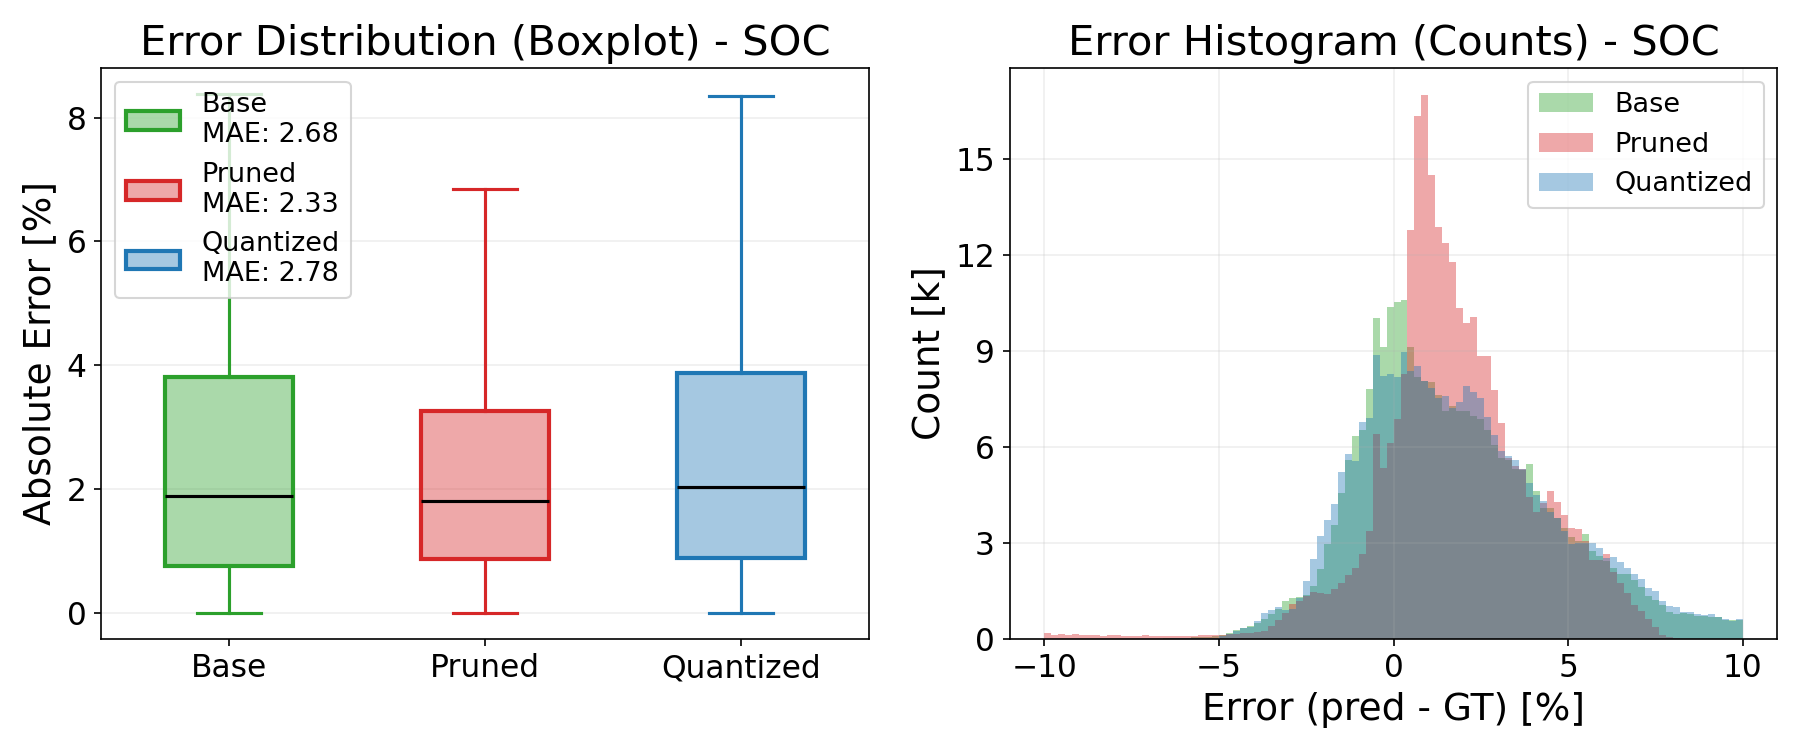
\includegraphics[width=\columnwidth]{figures/Combined_Results/Figure_9_SOC_MAE_Hist.png}
    \caption{SOC Error Analysis: MAE distribution (left) and error histogram (right). The tight clustering around zero confirms unbiased estimation.}
    \label{fig:soc_error}
\end{figure}
\begin{figure}[tbp]
    \centering
    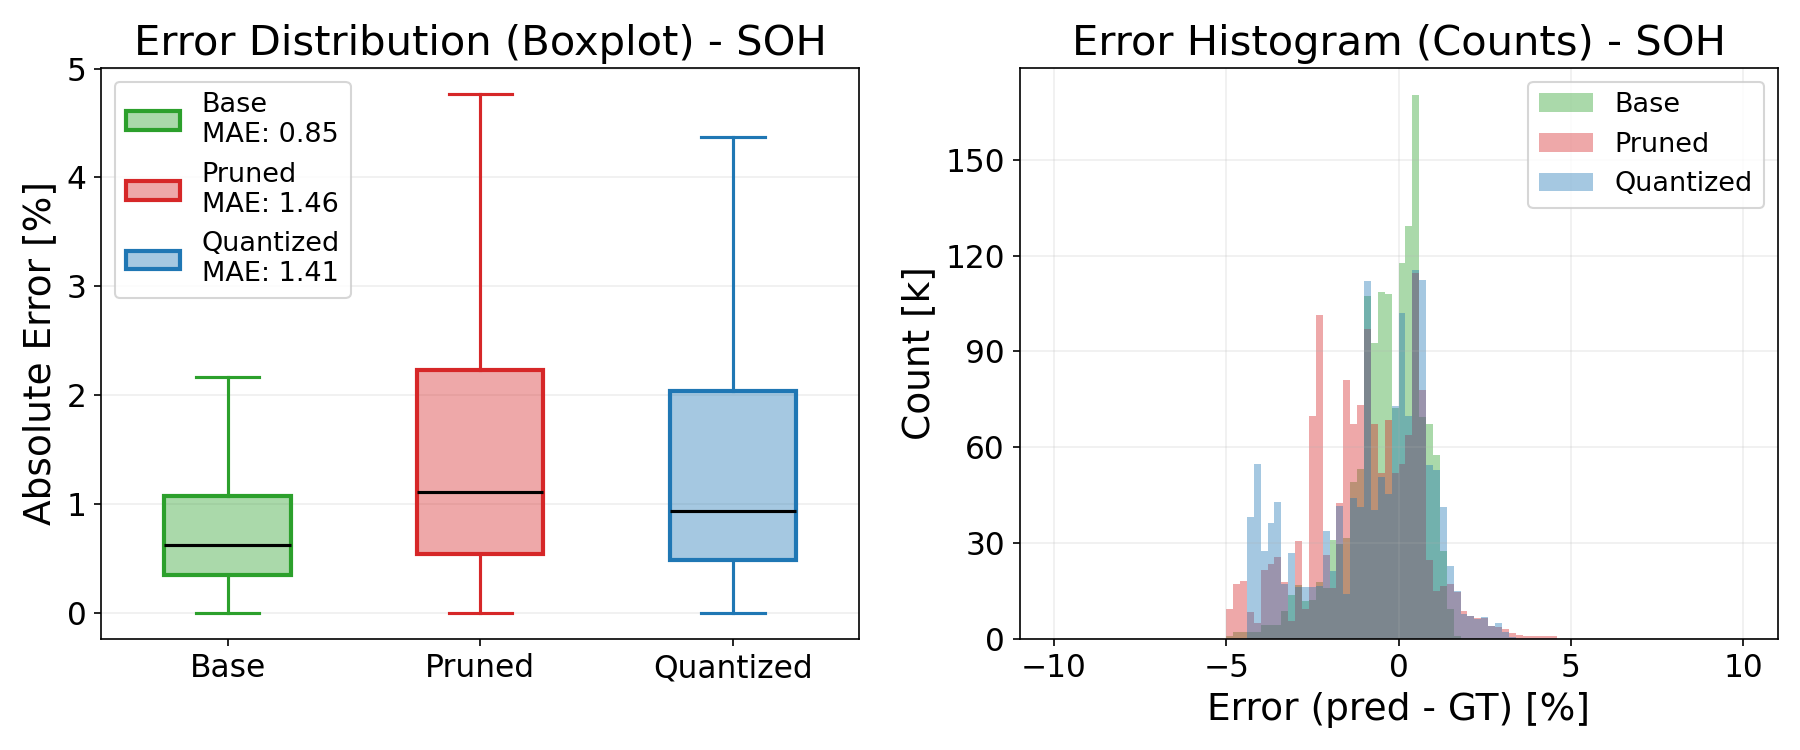
\includegraphics[width=\columnwidth]{figures/Combined_Results/Figure_10_SOH_MAE_Hist.png}
    \caption{SOH Error Analysis: MAE distribution (left) and error histogram (right). The spread is naturally larger due to the difficulty of the task, yet the quantized model remains robust.}
    \label{fig:soh_error}
\end{figure}
\begin{figure*}[t!]
    \centering
    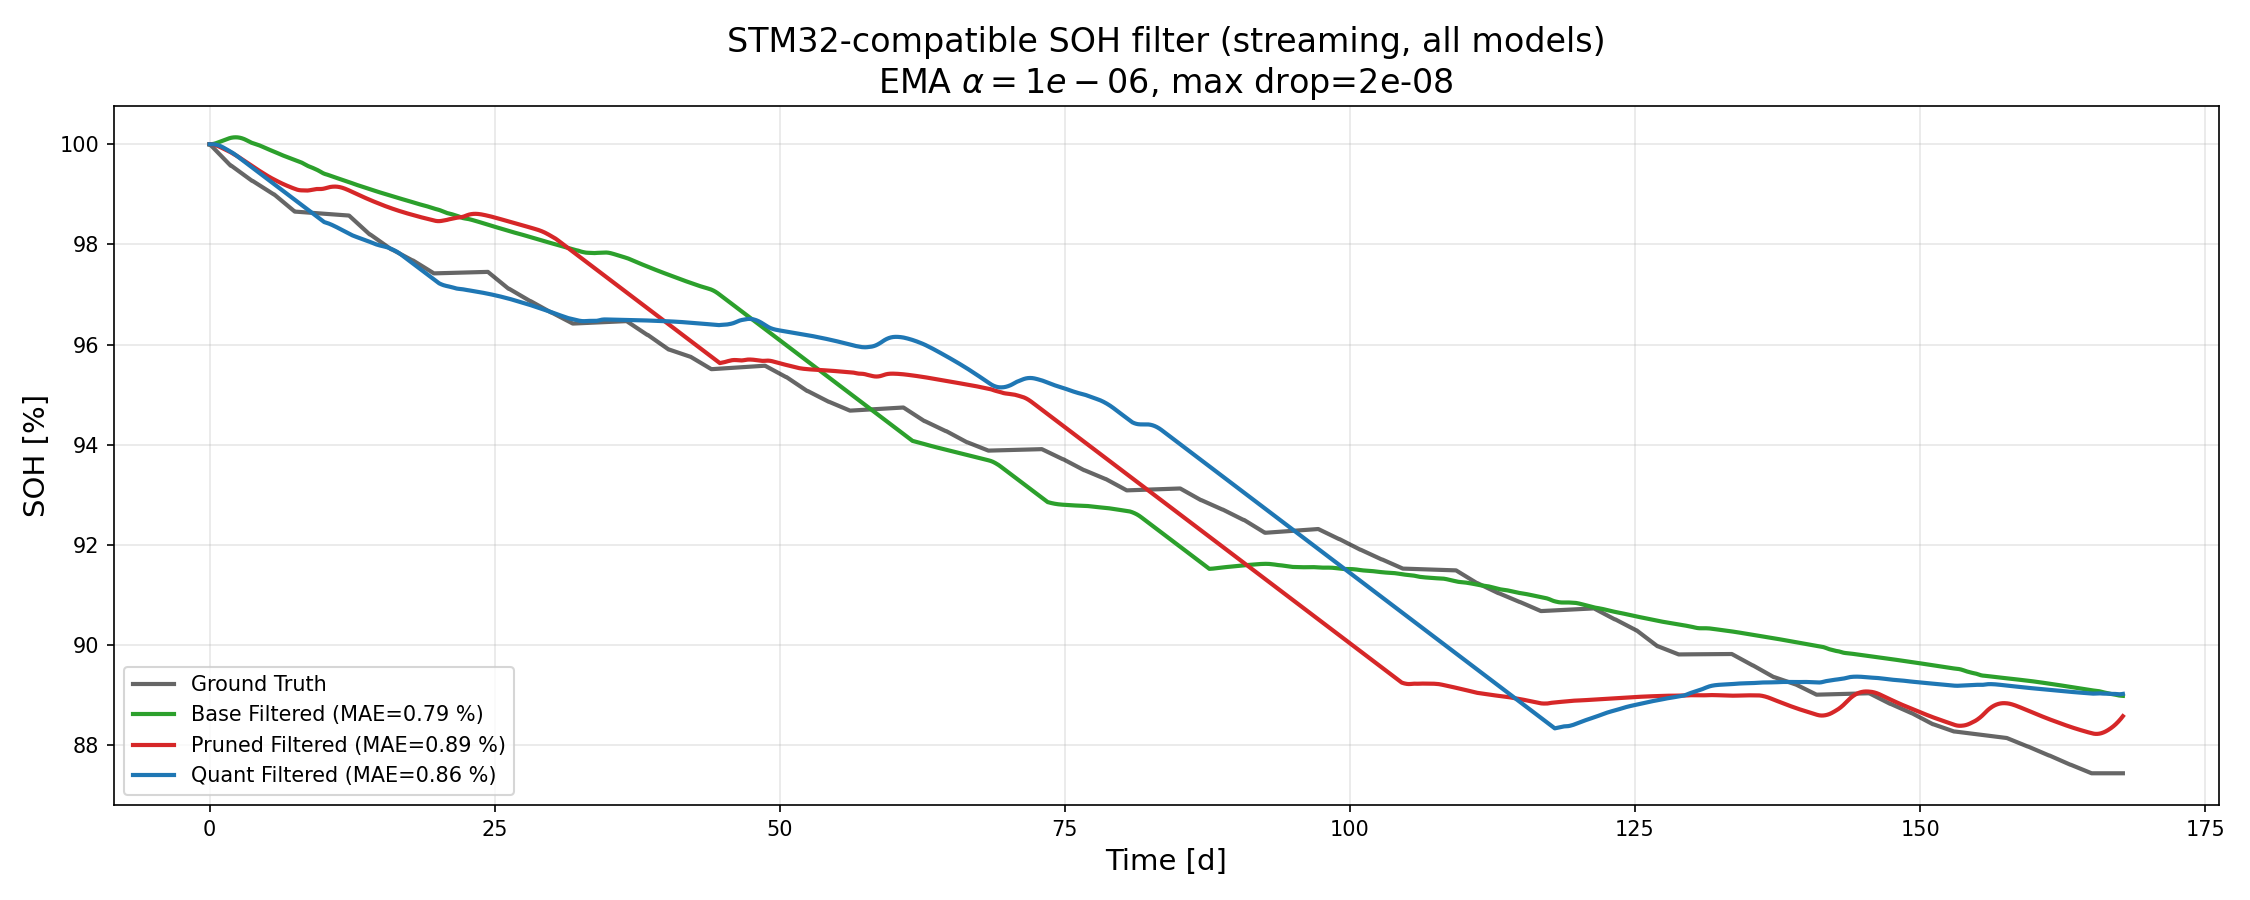
\includegraphics[width=\textwidth]{figures/Combined_Results/Figure_11_SOH_Streaming_Dashboard.png}
    \caption{Streaming SOH dashboard with online filtering. The top panel shows the reference SOH and the outputs of the Base (green), Pruned (red), and Quantized (blue) models; the bottom panel depicts the corresponding prediction errors after causal smoothing.}
    \label{fig:soh_dashboard}
\end{figure*}
\subsection{Error Distribution Analysis}
To quantify the reliability of the estimators, we analyse the statistical distribution of the prediction errors. Figures~\ref{fig:soc_error} and~\ref{fig:soh_error} present the Mean Absolute Error (MAE) boxplots and the error histograms for both tasks.
The SOC error distribution is remarkably narrow and symmetric, indicating no systematic bias. The boxplots reveal that the pruned model attains the smallest median MAE and interquartile range with respect to the reference SOC, while the quantized model closely matches the full-precision baseline. Pruning thus provides a slight accuracy gain at reduced runtime, whereas quantization preserves the baseline behaviour with a markedly smaller weight footprint, offering a complementary operating point when flash capacity is the primary constraint.
For SOH, the error distribution is broader, which is inherent to the difficulty of estimating capacity fade from operational data. However, the histograms show that the bulk of the errors are still contained within a useful tolerance band (typically $\pm 2\%$), making the embedded estimator a viable tool for onboard diagnostics.
\subsection{Transient Response and Zoomed Analysis}
Global metrics often hide local failures. To inspect the transient behaviour, we zoom into a high-dynamic pulse discharge phase (Fig.~\ref{fig:zoom_pulse}) and into a representative check-up sequence (Fig.~\ref{fig:zoom_checkup}).
\par
In the pulse region (Fig.~\ref{fig:zoom_pulse}), the models must react to rapid current changes. The quantized model follows the ground truth transients with high fidelity, capturing the voltage recovery phases accurately. The pruned model, having fewer parameters to model the complex electrochemical relaxation, tends to smooth out these sharp features slightly.
\begin{figure*}[t!]
    \centering
    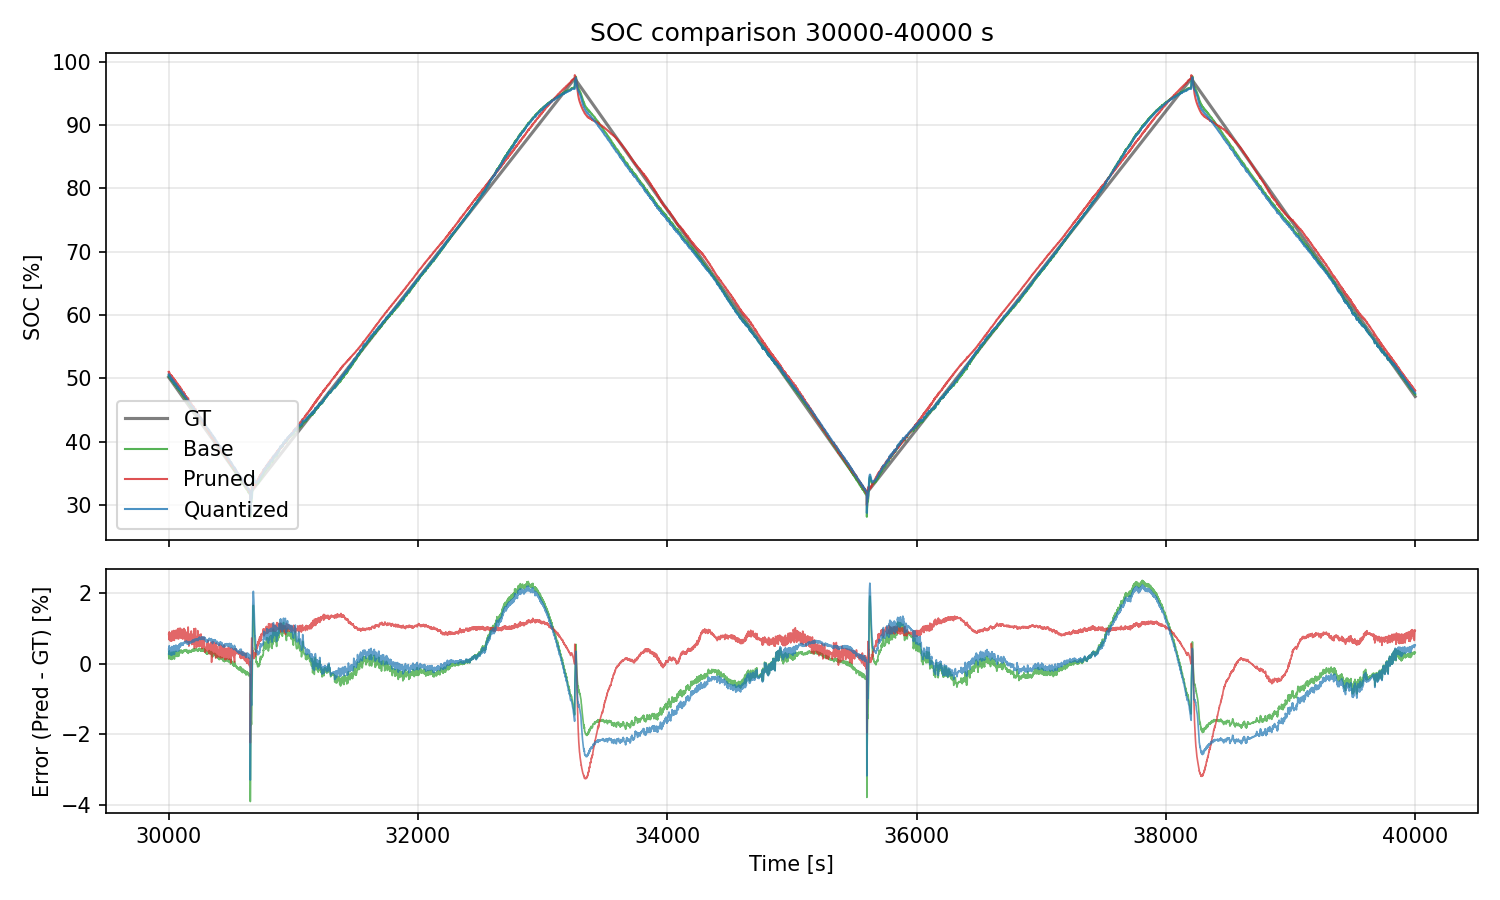
\includegraphics[width=\textwidth]{figures/Combined_Results/Figure_12_SOC_Zoom_Pulse.png}
    \caption[Transient response (pulse segment)]{Detailed transient analysis of SOC streaming replay (pulse segment). Response to dynamic load pulses (30k--40k\,s).}
    \label{fig:zoom_pulse}
\end{figure*}
\begin{figure*}[t!]
    \centering
    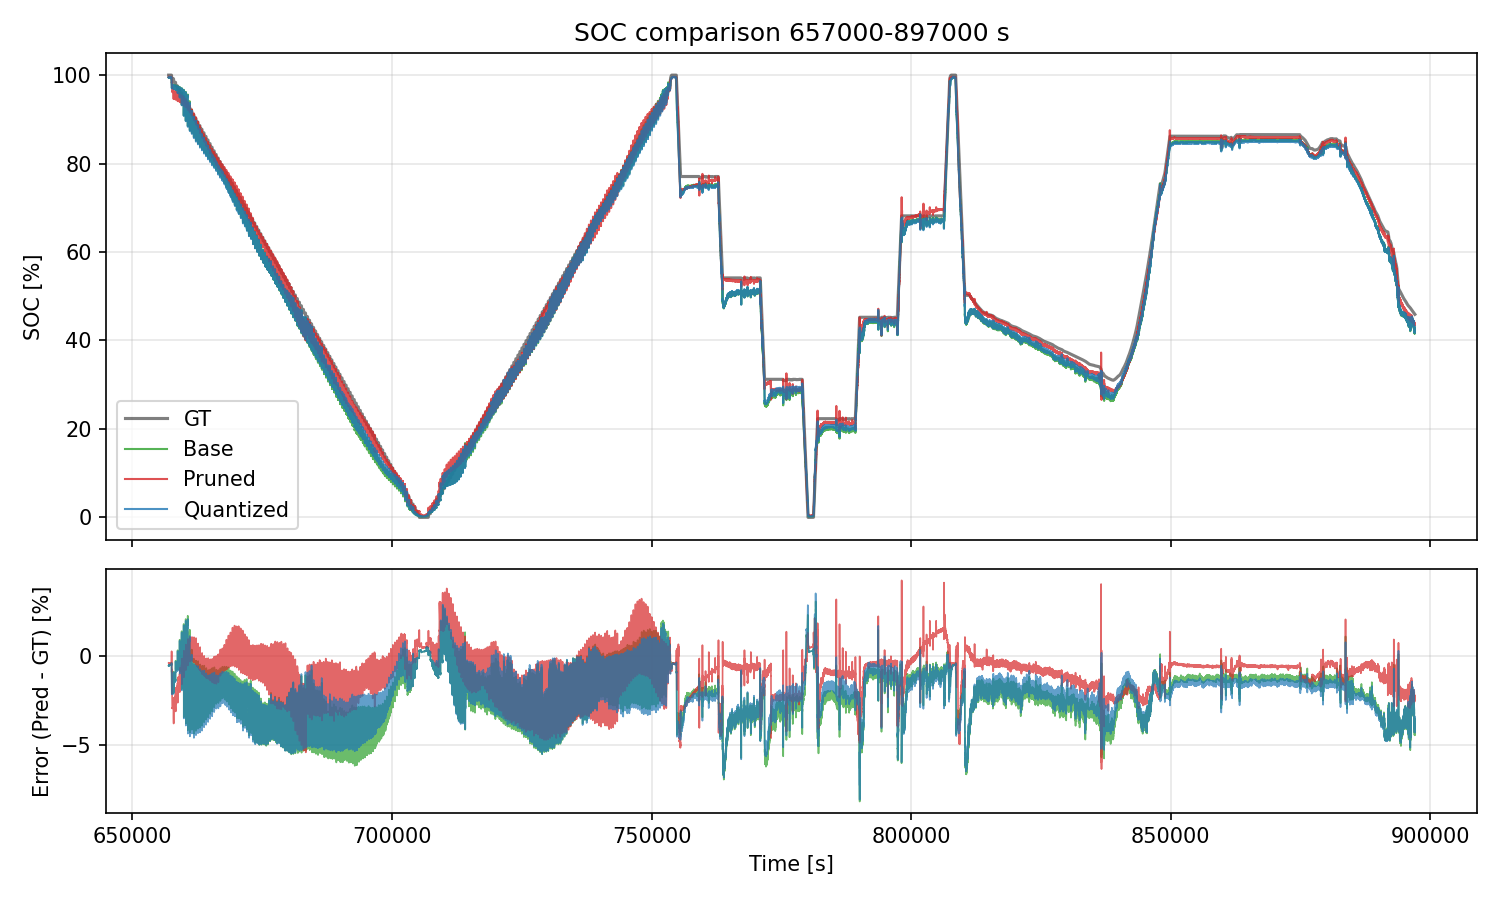
\includegraphics[width=\textwidth]{figures/Combined_Results/Figure_13_SOC_Zoom_Checkup.png}
    \caption[Transient response (check-up segment)]{Detailed transient analysis of SOC streaming replay (check-up segment). Behaviour during a capacity check-up (657k--897k\,s).}
    \label{fig:zoom_checkup}
\end{figure*}
\noindent
During the check-up phase (Fig.~\ref{fig:zoom_checkup}), where the cell undergoes full charge/discharge cycles, all models converge well, demonstrating stability over long integration horizons.
\subsection{Resource Efficiency and Latency}
Finally, we evaluate the cost of deployment. Figures~\ref{fig:resources_sizes} and~\ref{fig:resources_latency} summarize the flash memory, RAM usage, and parameter counts for both SOC and SOH models and the corresponding latency distribution on the STM32H7 microcontroller.
For all deployments the model complexity is first characterised on the workstation side by counting parameters in each variant (base, pruned, quantized). Assuming four bytes per weight for floating point representations and one byte per weight for INT8, this directly yields an estimate of the flash footprint attributable to the neural network weights alone. The second stage of the analysis uses the linker map files of the STM32CubeIDE projects to determine the actual binary size in flash, which also includes code, constant tables, and run-time support libraries. This explains why the measured flash usage in Figure~\ref{fig:resources_sizes} is systematically higher than the idealised "weights only" estimate, and why the gap is larger for the more complex SOH firmware that contains additional diagnostic and filtering logic.
The RAM usage shown in the lower right panel of Figure~\ref{fig:resources_sizes} is obtained from on-device measurements of the SOH and SOC firmware and applied analogously to all STM32 deployments. At boot time the firmware reports the size of the statically allocated data and BSS sections, which correspond to persistent variables and network parameters stored in SRAM. During each benchmark inference the minimum value of the stack pointer is tracked, so that the maximum additional stack consumption of the call chain can be recovered. The total RAM requirement reported in the figure is the sum of static data and worst-case stack usage, i.e.\ an upper bound on the memory needed to execute one inference including the LSTM state updates and UART handling. This procedure captures the fact that pruning reduces both the number of parameters and the amount of intermediate state that must be kept in memory, whereas quantization primarily reduces the storage needed for the weights and activations, with a smaller impact on the stack frame size.
The bar charts in Figure~\ref{fig:resources_sizes} clearly highlight the benefits of the optimisation pipeline. The quantized models (blue bars) achieve a dramatic reduction in Flash usage compared to the baseline (green), bringing the complex SOH model down to a footprint that comfortably fits alongside the SOC estimator on a mid-range MCU. Pruning (red bars) is particularly effective at reducing the parameter count and RAM usage, which directly translates to shorter execution times.
\begin{figure*}[tb]
    \centering
    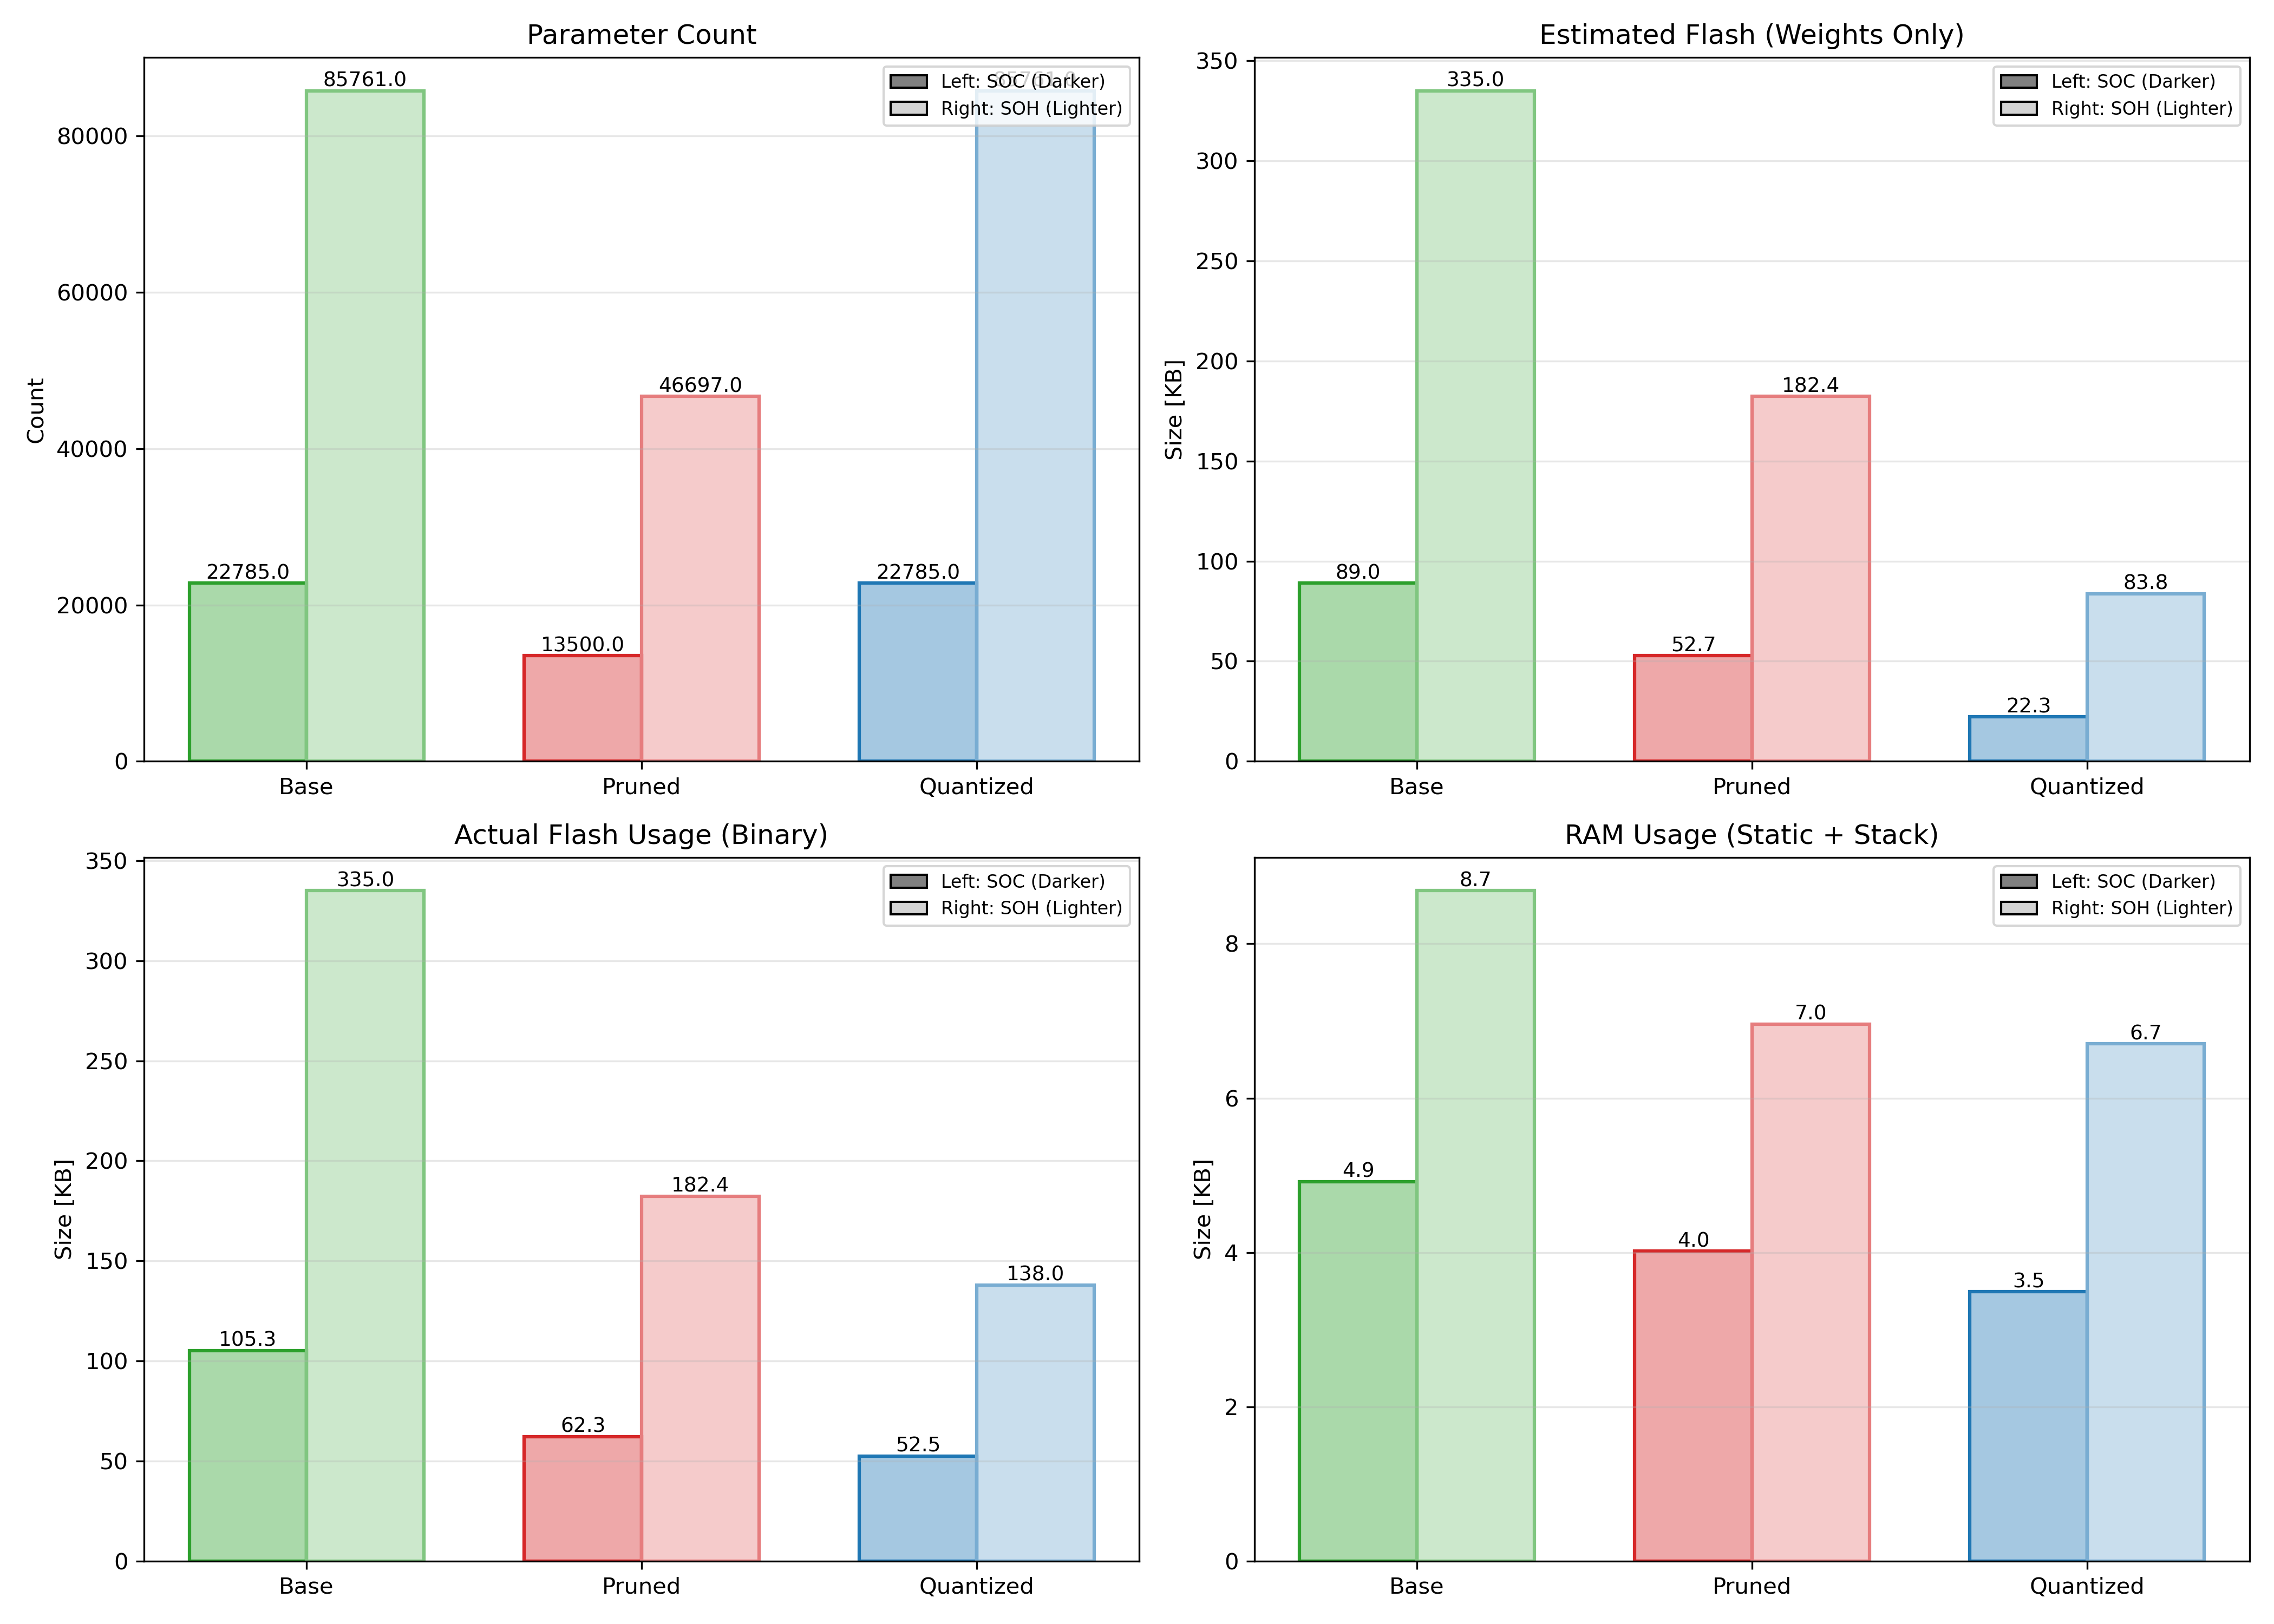
\includegraphics[width=\textwidth]{figures/Combined_Results/Figure_14_Model_Sizes.png}
    \caption{Resource landscape for SOC and SOH models. Comparison of parameter count, estimated Flash, actual Flash, and RAM usage. Dark bars denote SOC, light bars denote SOH.}
    \label{fig:resources_sizes}
\end{figure*}

\noindent
Figure~\ref{fig:resources_latency} reports the corresponding host-side latency distributions.
\begin{figure}[tbp]
    \centering
    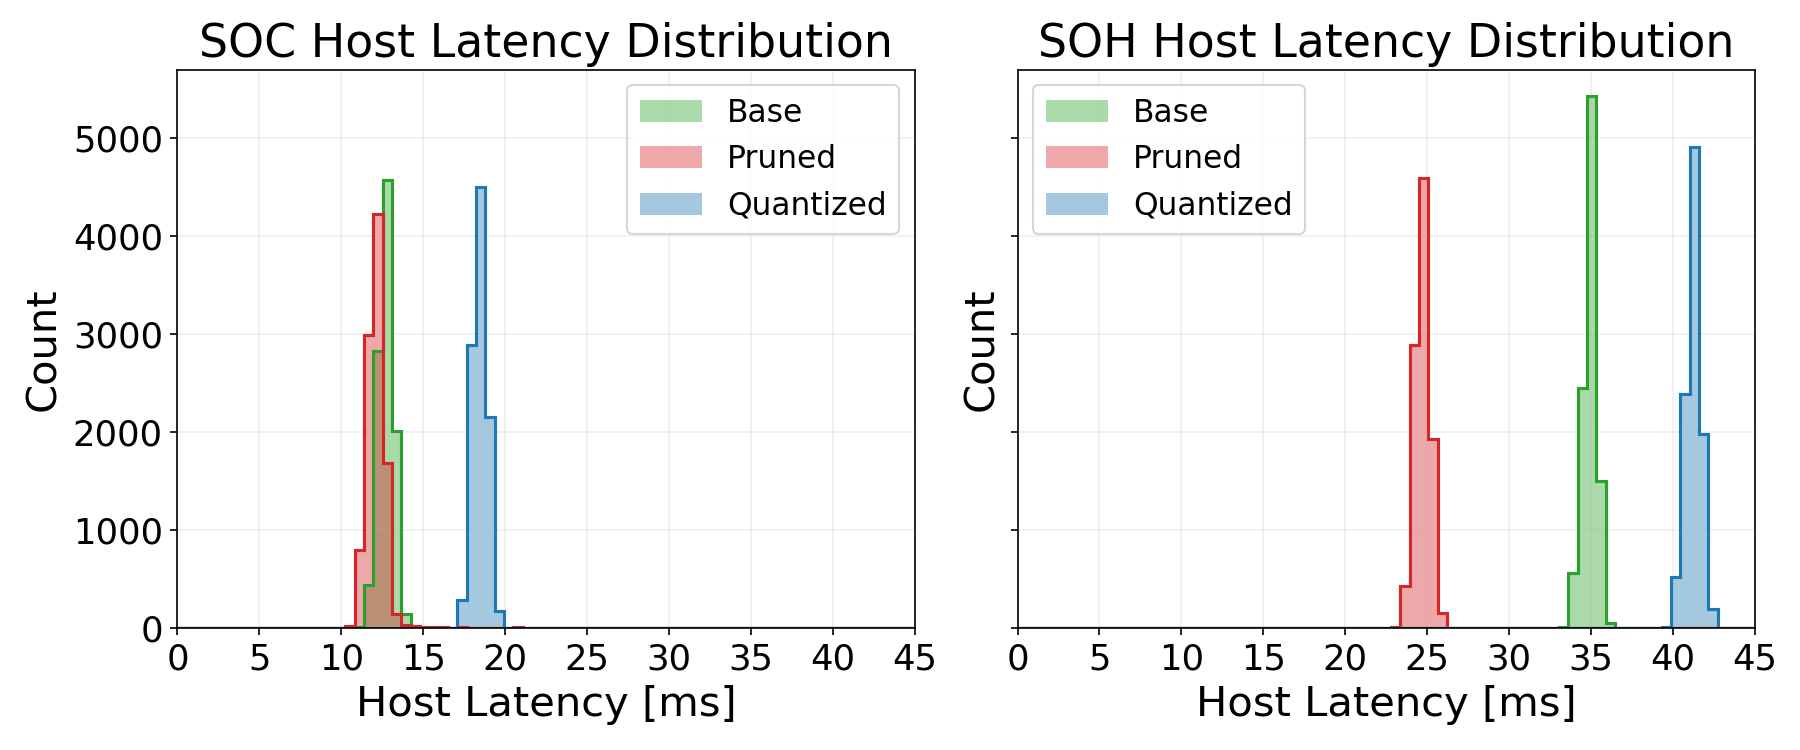
\includegraphics[width=\columnwidth]{figures/Combined_Results/Figure_15_Latency_Hist.png}
    \caption{Latency distributions for SOC and SOH models on the STM32H7. Histograms are computed from repeated on-device measurements.}
    \label{fig:resources_latency}
\end{figure}
The latency distributions in Figure~\ref{fig:resources_latency} reveal a distinct hierarchy that is consistent with the model sizes. On the inference side, the SOC estimators execute in approximately \SIrange{0.8}{7}{\milli\second} depending on the compression strategy, whereas the SOH variants require on the order of \SIrange{12}{30}{\milli\second} per update. The fully quantized SOC deployment is the slowest in terms of pure inference time because the INT8 weights are unpacked inside a hand-written kernel, yet even here the computation remains well below \SI{10}{\milli\second}. When the host-side communication overhead (UART framing and Python processing) is included, the end-to-end latencies remain below roughly \SI{20}{\milli\second} for all SOC models and below \SI{50}{\milli\second} for the SOH estimator, which is comfortably within the sampling periods of typical stationary storage BMS and low-rate diagnostic tasks. This analysis allows engineers to quantify the trade-off between compression, model complexity, and timing margin on a concrete MCU target.
\subsection{Composite trade-off summary}
To make the multi-objective trade-offs easier to interpret at a glance, we report a simple composite utility score $U$ that aggregates accuracy and embedded resource indicators into a single, dimensionless index. For a given task (SOC or SOH) and a model variant $v$, we define
\begin{equation}
\label{eq:utility_u}
U_v = \frac{1}{4}\left(
\frac{\mathrm{MAE}_v}{\mathrm{MAE}_{\mathrm{Base}}} +
\frac{F_v}{F_{\mathrm{Base}}} +
\frac{R_v}{R_{\mathrm{Base}}} +
\frac{E_v}{E_{\mathrm{Base}}}
\right),
\end{equation}
where $\mathrm{MAE}$ is the streaming mean absolute error (in \% of full scale), $F$ is the measured flash footprint, $R$ the measured total RAM usage (static + peak stack), and $E$ the measured energy per inference on the STM32. By construction $U_{\mathrm{Base}}=1$; values $U<1$ indicate that a variant improves, on average, across these four objectives. The score is intended as an illustrative summary only: deployments can prioritise objectives differently, which can be reflected by replacing the equal weighting in~\eqref{eq:utility_u} with task-specific weights.
Table~\ref{tab:tradeoff_summary} summarises the resulting changes for pruning and quantization; values are reported as SOC/SOH.
\begin{table}[tbp]
    \centering
    \caption[Summary of pruning/quantization effects]{At-a-glance effect of pruning and quantization relative to the corresponding Base model. Values are reported as SOC/SOH. $\Delta$MAE is reported in percentage points (pp) of full scale (negative indicates improved accuracy); flash, RAM, and energy changes are relative deltas versus Base. The composite score $U$ follows~\eqref{eq:utility_u} (lower is better). In this study pruning is the most effective lever for reducing energy, whereas quantization is the most effective lever for reducing flash.}
    \label{tab:tradeoff_summary}
    \scriptsize
    \setlength{\tabcolsep}{2.5pt}
    \renewcommand{\arraystretch}{1.05}
    \begin{tabular}{lccccc}
        \toprule
        Variant & $\Delta$MAE [pp] & $\Delta$Flash [\%] & $\Delta$RAM [\%] & $\Delta$Energy [\%] & $U$ \\
        \midrule
        Pruned & \textcolor{mgGreen}{-0.35}/\textcolor{mgRed}{+0.61} & \textcolor{mgGreen}{-41}/\textcolor{mgGreen}{-46} & \textcolor{mgGreen}{-18}/\textcolor{mgGreen}{-20} & \textcolor{mgGreen}{-43}/\textcolor{mgGreen}{-44} & 0.71/0.91 \\
        Quantized & \textcolor{mgRed}{+0.10}/\textcolor{mgRed}{+0.56} & \textcolor{mgGreen}{-50}/\textcolor{mgGreen}{-59} & \textcolor{mgGreen}{-20}/\textcolor{mgGreen}{-23} & \textcolor{mgRed}{+399}/\textcolor{mgRed}{+29} & 1.83/1.03 \\
        \bottomrule
    \end{tabular}
\end{table}

\section{Discussion}
The experiments show that pruning and quantization affect the SOC and SOH estimators in different ways. For SOC, both the streaming plots and the error histograms indicate that compression can be applied without sacrificing estimation quality. The pruned SOC model achieves a slightly lower MAE and a narrower error distribution than the dense baseline, which is consistent with an over-parameterised 64-unit LSTM in which pruning primarily removes redundant units and acts as an additional regulariser. The quantized SOC model tracks both the baseline and the reference SOC almost indistinguishably in the long-horizon replay, with discrepancies that remain within the numerical noise introduced by the FP32 de-quantization.

For SOH the picture is more nuanced. The SOH targets evolve slowly, are observed reliably only during periodic capacity check-ups, and the online estimator operates on filtered signals. In this setting the 128-unit baseline uses its capacity more effectively, and both pruning and quantization introduce a noticeable but still bounded loss in accuracy. The error histograms exhibit broader tails for the compressed SOH models and do not reveal a clear winner between pruning and INT8. This behaviour is compatible with the higher intrinsic noise level of the SOH regression task and suggests that aggressive compression should be combined with additional temporal filtering or architectural changes if very small error margins are required.

From an engineering perspective the three deployment variants represent distinct operating points. The base FP32 model offers the simplest tool flow but requires the largest flash footprint and the longest on-device execution time. Pruning reduces the recurrent state dimension and the associated MLP rows, shrinking the SOC flash usage from about 105~kB to 62~kB and shortening the on-device inference time from 1.40~ms to 0.80~ms (roughly 40~\%). For the SOH estimator the corresponding numbers are 335~kB to 182~kB and 22.73~ms to 12.72~ms, respectively. Quantization, in turn, achieves the smallest flash and RAM footprint, with the SOC weight storage reduced by approximately a factor of four compared with FP32. On the STM32H7 this comes at the cost of additional de-quantization work inside the hand-written kernels: the quantized SOC model reaches 6.99~ms inference time, while the quantized SOH model trades part of the runtime gains of pruning for a further reduction in flash usage. Because the compressed deployments still meet real-time constraints with ample margin, the choice between pruned and quantized variants can be guided by the available flash budget and the strictness of the latency targets.

The distinction between system latency and inference time is particularly relevant for resource-constrained BMS. The UART-driven tests report end-to-end latencies between roughly 12~ms and 18~ms for the SOC variants and between 25~ms and 40~ms for the SOH models, values that are dominated by serial communication and host scheduling. The on-device inference times in Tables~\ref{tab:kpi} and~\ref{tab:kpi_soh}, by contrast, show that the SOC estimator requires less than 1.5~ms of compute time per sample, while the SOH estimator completes one update in approximately 23--30~ms. Typical sampling rates for pack-level monitoring in stationary storage and EV battery management systems lie in the single-digit to low double-digit hertz range~\cite{plettBatteryManagementSystems2015,berecibarCriticalReviewState2016}, so all investigated deployments satisfy real-time constraints with comfortable margin.

More generally, the reported measurements describe a multi-objective trade-off space rather than a single ``best'' solution. In practical BMS deployments, accuracy, flash, RAM, and energy cannot typically be minimised simultaneously, so application-specific priorities and constraints must be specified explicitly. A pragmatic way to use our results is therefore constraint-driven: impose acceptable accuracy bounds (e.g., MAE/RMSE ceilings) together with hard memory budgets (flash/RAM), and then select the candidate that minimises energy per inference among the feasible models. If a single scalar ranking is desired, the normalised utility score $U$ presented in Table~\ref{tab:tradeoff_summary} offers a compact comparison. For the SOC estimator, the pruned variant achieves the most favourable score ($U=0.71$), reflecting substantial gains in both efficiency and accuracy. In contrast, the quantized SOC model yields a score of $U=1.83$ despite its minimal footprint, as the software-based de-quantization overhead significantly increases energy consumption. For the SOH task, both compressed models hover near the baseline utility ($U \approx 0.9$--$1.0$), indicating that the flash savings are roughly balanced by the slight degradation in accuracy and the overhead of the INT8 kernel. This underscores that while quantization is the most effective tool for minimising flash usage, pruning currently offers a more balanced profile for energy-constrained software implementations on the STM32H7.

Current limitations include the focus on a single, albeit rich, experimental campaign from the LFP DoE Cycle Ageing Dataset, the restriction to one cell chemistry, and the lack of a systematic study on measurement noise, sensor drift, or fault injection on the embedded platform.
\section{Conclusion and Outlook}
This work presents a complete and reproducible path from data-driven SOC and SOH estimators to an STM32-based battery management controller. Starting from LSTM\,+\,MLP models trained on the LFP DoE Cycle Ageing Dataset, we derive pruned and quantized variants and benchmark all deployments with respect to accuracy, timing, memory usage, and energy on an STM32H753ZI microcontroller.

For SOC, the experiments show that aggressive compression is possible without sacrificing estimation quality. The pruned SOC model reduces the recurrent state dimension while slightly improving MAE and narrowing the error distribution, and it lowers both the flash footprint and the energy per inference by roughly 40~\% compared to the full-precision baseline. Quantization further shrinks the weight storage to about half of the original size and keeps the SOC accuracy within numerical distance of the full-precision model, but it increases the energy per inference because of the additional de-quantization work in the hand-written kernels. For SOH, pruning and quantization follow the same qualitative trends: flash savings on the order of 45--60~\% and energy reductions of about 45~\% for the pruned variant. The resulting accuracy/complexity trade-off is more modest because the underlying regression problem is noisier and driven by sparse capacity measurements.

The resource and latency measurements demonstrate that all investigated deployments meet typical real-time constraints for stationary storage applications by a comfortable margin, and that co-location of SOC and SOH estimators on a single STM32H7 is feasible even for the high-capacity SOH model. The methodology, including the quantization scheme, firmware integration, and benchmarking scripts, can be reused to compare alternative SOC/SOH estimators on equal footing.


\section*{Declaration of generative AI and AI-assisted technologies in the manuscript preparation process}
During the preparation of this work the authors used ChatGPT, DeepL, and Grammarly in order to improve the language and style of the manuscript. After using these tools/services, the authors reviewed and edited the content as needed and take full responsibility for the content of the published article.

Future work will focus on transferring the embedded estimators from the evaluation board to a full battery management system with pack-level integration, where additional constraints such as communication bandwidth and safety monitoring become critical. On the modelling side it will be important to extend the study to additional cell chemistries, temperature ranges, and loading regimes, and to compare the LSTM backbone against alternative architectures such as GRUs, Transformers, or hybrid observers that combine equivalent-circuit models with neural components~\cite{liptonCriticalReviewRecurrent2015,singhDeepMachineLearning2024,gaoEnhancedStateofchargeEstimation2022,wangFusionEstimationLithiumion2022}. Another promising direction is to jointly tune pruning and quantization, combining the low memory footprint of INT8 weights with the computational efficiency of sparse connectivity. Specifically, quantizing an already pruned model could yield a synergistic effect, minimizing both Flash storage and execution time simultaneously. This would allow for even more compact deployments on ultra-low-power microcontrollers where both memory and compute cycles are scarce. These extensions will clarify how far the presented optimisation strategy generalises and where further algorithmic advances are required for next-generation resource-aware BMS.
\section*{Data availability}
The LFP DoE Cycle Ageing Dataset used in this work can be obtained from the DOI repository in~\cite{LFP_DoE_Cycle_Aging_Dataset}. The landing page provides licensing information and download instructions.

\section*{Declaration of generative AI and AI-assisted technologies in the manuscript preparation process}
During the preparation of this work the author(s) used ChatGPT, DeepL, and Grammarly in order to improve the linguistic quality and style of the manuscript. After using these tools, the author(s) reviewed and edited the content as needed and take(s) full responsibility for the content of the published article.

\section*{Data availability}
The LFP DoE Cycle Ageing Dataset used in this work can be obtained from the DOI repository in~\cite{LFP_DoE_Cycle_Aging_Dataset}. The landing page provides licensing information and download instructions.

\bibliographystyle{elsarticle-num}
\bibliography{bib/paper2_socsoh_fr}
\end{document}

